\chapter{SOFR- Secured Overnight Financing Rate}
\label{chp_SOFR}

\section{Introduction}
Following the LIBOR scandal, the Federal Reserve and regulators in the U.K. have come up with a replacement called the Secured Overnight Financing Rate (SOFR) \nomenclature{SOFR}{Secured Overnight Financing Rate}.
There are also other RFR alternatives (Risk-Free Reference Rates) \nomenclature{RFR}{Risk-Free Reference Rates} who work similarly: SONIA (Sterling Overnight Index Average) 
\nomenclature{SONIA}{Sterling Overnight Index Average} managed by The Bank of England. One could also mention €STR (Euro Short-Term Rate) \nomenclature{€STR}{Euro Short-Term Rate}
\cite{CME_SOFR}.
\\~\\
On November 30, 2020, the Federal Reserve announced that the LIBOR would be phased out and eventually replaced by June 2023. Banks were also instructed to stop writing contracts using the LIBOR by the end of 2021, and that all contracts using the LIBOR should wrap up by June 30, 2023 \cite{hayes_2022}.
\\~\\ 
SOFR is fundamentally different from LIBOR. The Federal Reserve Bank of New York collects transaction data from the overnight Treasury Repo market. It then calculates a volume-weighted median interest rate. Which then gets published at 08.00 AM (Eastern Time) the following business day \cite{ARRC_SOFR}.
\\~\\ 
This means that SOFR is backwards looking as it is based upon overnight transactions. Furthermore, it cannot look beyond 24 hours.  
\\~\\
\textbf{Key differences between LIBOR and SOFR/RFR's}

\begin{enumerate}
    \item Calculation Method: LIBOR is calculated based on submissions from Panel Banks. SOFR is based on the overnight repo market. 
    \item Tenors: LIBOR has multiple tenors, while SOFR has one: overnight. Meaning that LIBOR is forward-looking while SOFR is backwards-looking. 
    \item Validity: Following the LIBOR scandal, one has seen that LIBOR has been more prone to manipulation, as one can give higher or lower rate submissions altering the trimmed mean. SOFR is transaction based, meaning that it is harder to manipulate. 
    \item Secured vs unsecured. Any collateral does not back up the loans that involve LIBOR. In the SOFR situation, the repo transaction is collateralized by a high-quality bond such as a US-Treasury note \cite{huggins2022sofr}. 
\end{enumerate}

\newpage 

\begin{definition}[\textbf{Discrete overnight SOFR \cite{Skov_2020}}]
The discrete overnight SOFR is defined as:
\[
R_{d_{i}}(T_{i}) = \frac{1}{d_{i}}\left(
\frac{1}{P(T_{i}, T_{i}+d_{i})} - 1
\right)
\]
Where:
\begin{itemize}[leftmargin=*]
    \item $d_{i}$: denotes the day count fraction multiplied by the number of days the overnight rate applies. I.e. $d_{i} = 1/360$ on business days, and $d_{i} = 3/360$ on fridays. 
\end{itemize}
\end{definition}

\begin{comment}
\begin{definition}[\textbf{SOFR 1-month arithmetic average \cite{Skov_2020}}]
The 1-month \nomenclature{1M}{1-month}
SOFR arithmetic average of the daily reference rate observed over the period $[S,T]$ is defined as: 
\[
R^{1M}(S,T) = \frac{1}{N}\sum_{i=1}^{N}R_{d_{i}}(T_{i})
\]
Where:
\begin{itemize}[leftmargin=*]
    \item $N$: total number of days in the month
    \item $S\leq T_{1} \leq \dots \leq T_{N} \leq T$ 
\end{itemize}
\end{definition}

\begin{definition}[\textbf{SOFR 3-month geometric average
\cite{Skov_2020}}]
The 3-month \nomenclature{3M}{3-months}
SOFR geometric average of the daily reference rate observed over the period $[S,T]$ is defined as: 
\[
R^{3M}(S,T) = \frac{1}{T-S}\left(
\prod_{i=1}^{N}(1+d_{i}R_{d_{i}}(T_{i})) - 1
\right)
\]
\end{definition}
\end{comment}

\begin{definition}[\textbf{Backward-looking compounding SOFR-average \cite{Skov_2020}}]
\label{def: backward_looking_SOFR_avg}
The backwards-looking compounded average over the period $[S,T]$ is defined as: 
\begin{align*}
R^{B}(S,T) &= \frac{1}{T-S}\left(
\prod_{i=1}^{N}[1+d_{i}R_{d_{i}}(T_{i})] - 1
\right)    
\end{align*}
\begin{itemize}[leftmargin=*]
    \item $N$: total number of days in the applicable period.
    \item $S\leq T_{1} \leq \dots \leq T_{N} \leq T$ 
\end{itemize}
\end{definition}

\begin{figure}[htp]
    \centering
    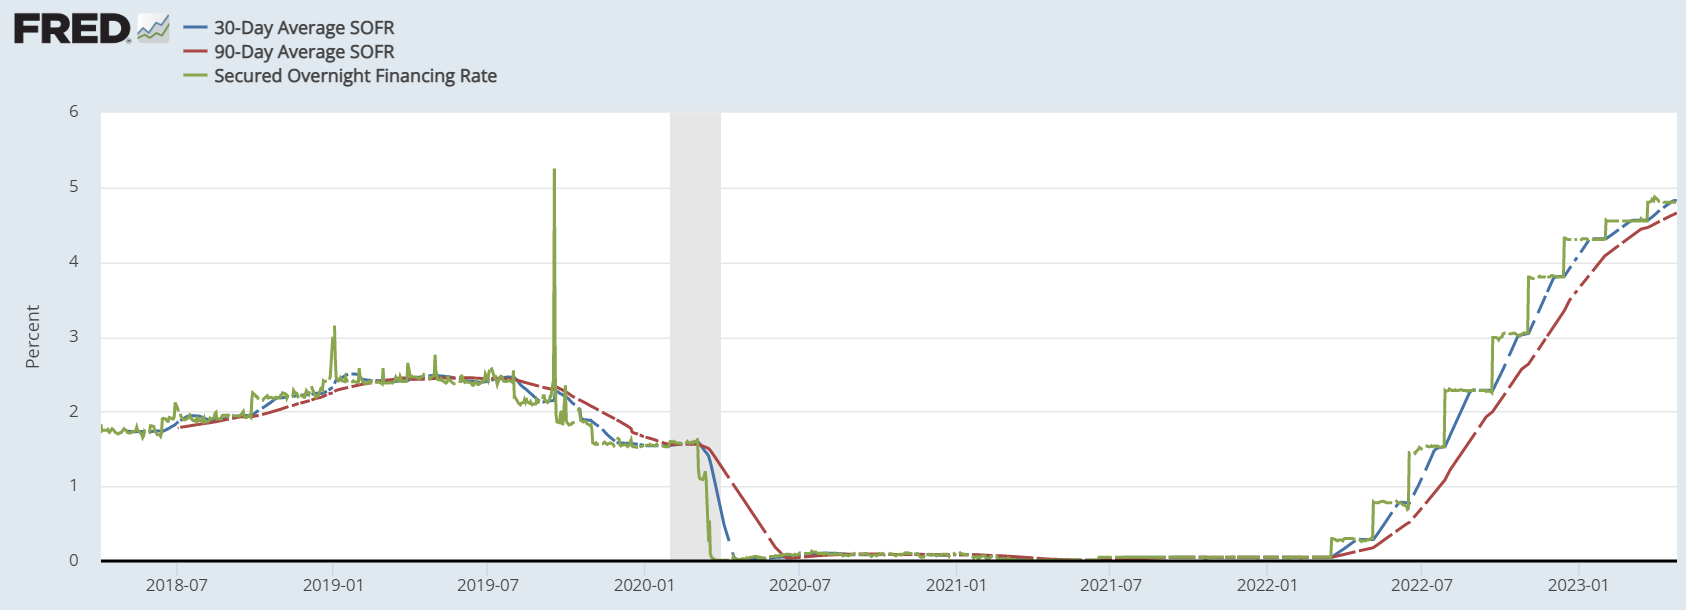
\includegraphics[height = 8cm, width=16cm]{figures/SOFR/ON_1M_3M_SOFR.PNG}
    \caption{O/N, 1M and 3M SOFR-rates}
    \label{fig: ON_1M_3M_SOFR}
\end{figure}

This figure is collected from \cite{FredSOFR} 
and displays the following SOFR rates:
green: O/N, blue: 1M-average and red: 3M-average. Here the 1M-average and 3M-average are calculated according to Definition \ref{def: backward_looking_SOFR_avg}. 
\\~\\
If we look at the green O/N rates, we see a spike in September 2019.  This was related to quarterly corporate tax payments due September 16. This led to a demand-supply mismatch  \cite{FederalReserve2019}.

\newpage 
As discussed in \cite{Skov_2020}, one has that $R^{B}(S,T)$ is $\F_{T}$-measurable. This is unsuitable as it does not incorporate market expectations about future rates. This leads to the following definition. 

\begin{definition}[\textbf{Forward-looking term-SOFR rate \cite{Skov_2020}}]
The forward-looking term SOFR rate over the period $[S,T]$ is defined as: 
\begin{align*}
R^{F}(S,T) &= \frac{1}{T-S}\left[
\frac{1}{P(S,T)} -1
\right]    
\end{align*}
\end{definition}

We see that the term SOFR rate is just a simple forward rate evaluated at time $t=S$ (See Definition \ref{def: Simple_forward_rate} p.\pageref{def: Simple_forward_rate}, i.e $R^{F}(S,T) = F(S,S,T)$). 

\begin{proposition}[\textbf{\cite{Skov_2020}}]
We have the following relationship between the forward-looking term SOFR rate $R^{F}(S,T)$ and the backwards-looking SOFR rate $R^{B}(S,T)$: 
\begin{align*}
R^{F}(S,T) &= \E_{Q^{T}}[R^{B}(S,T)|\F_{S}]    
\end{align*}
\end{proposition}

\begin{proof}

We start by calculating the expectation: 
\begin{align}
\label{eq: QT_expectation_R_Backwards}
\E_{Q^{T}}\left[
R^{B}(S,T)|\F_{S}
\right]
&= 
\E_{Q^{T}}\left[
\frac{1}{T-S}\left(
\prod_{i=1}^{N}[1+d_{i}R_{d_{i}}(T_{i})] - 1
\right)
\bigg{|}\F_{S}
\right] \nonumber \\ 
&= 
\frac{1}{T-S}
\left(\E_{Q^{T}}\left[
\prod_{i=1}^{N}[1+d_{i}R_{d_{i}}(T_{i})]\bigg{|}\F_{S} 
\right] - 1
\right)
\end{align}

Now: $R_{d_{i}}(T_{i}) = R^{F}(T_{i}, T_{i}+d_{i})$, this means that: 
\[
1 + d_{i}R_{d_{i}}(T_{i}) = \frac{1}{P(T_{i}, T_{i} + d_{i})}
\]

This yields:
\begin{align*}
\E_{Q^{T}}\left[
\prod_{i=1}^{N}[1+d_{i}R_{d_{i}}(T_{i})]\bigg{|}\F_{S} 
\right]
&= 
\E_{Q^{T}}\left[
\prod_{i=1}^{N}\frac{
1
}{
P(T_{i}, T_{i} + d_{i})
}
\bigg{|}\F_{S}
\right]
\end{align*}

For simplicity we let $T_{i+1} = T_{i} + d_{i}$, this gives us the following timeline:


\begin{tikzpicture}[snake=zigzag, line before snake = 5mm, line after snake = 5mm]
    % draw horizontal line   
    \draw (0,0) -- (3,0);
    \draw[snake] (3,0) -- (6,0);
    \draw (6,0) -- (9,0);

    % draw vertical lines
    \foreach \x in {0,3,6,9}
      \draw (\x cm,3pt) -- (\x cm,-3pt);

    % draw nodes
    \draw (0,0) node[below=3pt] {$ S = T_{1} $} node[above=3pt] {$   $};
    \draw (3,0) node[below=3pt] {$ T_{2} $} node[above=3pt] {$  $};
    \draw (6,0) node[below=3pt] {$ T_{N} $} node[above=3pt] {$  $};
    \draw (9,0) node[below=3pt] {$ T_{N+1} = T $} node[above=3pt] {$  $};
  \end{tikzpicture}

We observe that: 
\begin{align*}
P(S,T) = P(T_{1}, T_{N+1}) &= \prod_{i=1}^{N}P(T_{i}, T_{i+1})    
\end{align*}

This gives us:
\begin{align*}
\E_{Q^{T}}\left[
\prod_{i=1}^{N}\frac{
1
}{
P(T_{i}, T_{i} + d_{i})
}
\bigg{|}\F_{S}
\right]
&= 
\E_{Q^{T}}\left[
\frac{1}{P(S,T)}
\bigg{|}\F_{S}\right]
= \frac{1}{P(S,T)}
\end{align*}


\begin{comment}
We use the fact from Lemma \ref{lemma: T-discounted-S-discounted-bond} p.\pageref{lemma: T-discounted-S-discounted-bond}, that for $t\leq S \leq T$:
\begin{align*}
\frac{P(t,S)}{P(t,T)}\;\text{is a $Q^{T}$-martingale}    
\end{align*}

\newpage 

We iterate backwards and use that, for $i = 2, \dots, N$: 
\begin{align*}
\E_{Q^{T}}\left[
\frac{P(T_{i}, T_{i})}{P(T_{i}, T_{i+1})}
\bigg{|}\F_{T_{i-1}}\right] 
&= 
\frac{P(T_{i-1}, T_{i})}{P(T_{i-1}, T_{i+1})}
\end{align*}

This means that we now have: 
\begin{align*}
\E_{Q^{T}}\left[
\prod_{i=1}^{N}\frac{
P(T_{i}, T_{i})
}{
P(T_{i}, T_{i} + d_{i})
}
\bigg{|}\F_{S}
\right]
&= 
\E_{Q^{T}}\left[
\frac{1}{P(T_{1}, T_{2})}\prod_{i=2}^{N}\frac{P(T_{i-1}, T_{i})}{P(T_{i-1}, T_{i+1})}
\bigg{|}\F_{S}\right]
\end{align*}

We will now iterate further backwards and use the tower law until we eventually end up with $T_{1}$ in the 
denominator and numerator of the product sum, meaning that we end up with: 
\begin{align*}
\E_{Q^{T}}\left[
\prod_{i=1}^{N}\frac{
P(T_{i}, T_{i})
}{
P(T_{i}, T_{i} + d_{i})
}
\bigg{|}\F_{S}
\right]
&= 
\E_{Q^{T}}\left[
\frac{1}{P(T_{1}, T_{2})}
\prod_{i=2}^{N}\frac{P(T_{1}, T_{i})}{P(T_{1}, T_{i+1})}
\bigg{|}\F_{S}\right]
\end{align*}

We note that $T_{1} = S$, meaning that what's inside the expectation is $\F_{S}$-measurable, furthermore: 
\begin{align*}
\frac{1}{P(T_{1}, T_{2})}\prod_{i=2}^{N}\frac{P(T_{1}, T_{i})}{P(T_{1}, T_{i+1})}
&= 
\frac{1}{P(T_{1}, T_{N+1})} = \frac{1}{P(S,T)}
\end{align*}
\end{comment}
Plugging this into Equation \ref{eq: QT_expectation_R_Backwards}, yields: 
\begin{align*}
\E_{Q^{T}}\left[
R^{B}(S,T)|\F_{S}
\right] 
&= 
\frac{1}{T-S}
\left(
\frac{1}{P(S,T)} - 1
\right) := R^{F}(S,T)
\end{align*}
\end{proof}

\newpage 

It should also be mentioned that SOFR is closely related to EFFR (Effective Federal Funds Rate). This is an overnight rate reflecting the rate banks and depository institutions lend/borrow to maintain the reserve requirements given by the Federal Reserve.

\nomenclature{EFFR}{Effective Federal Funds Rate}
\begin{figure}[htp]
    \centering
    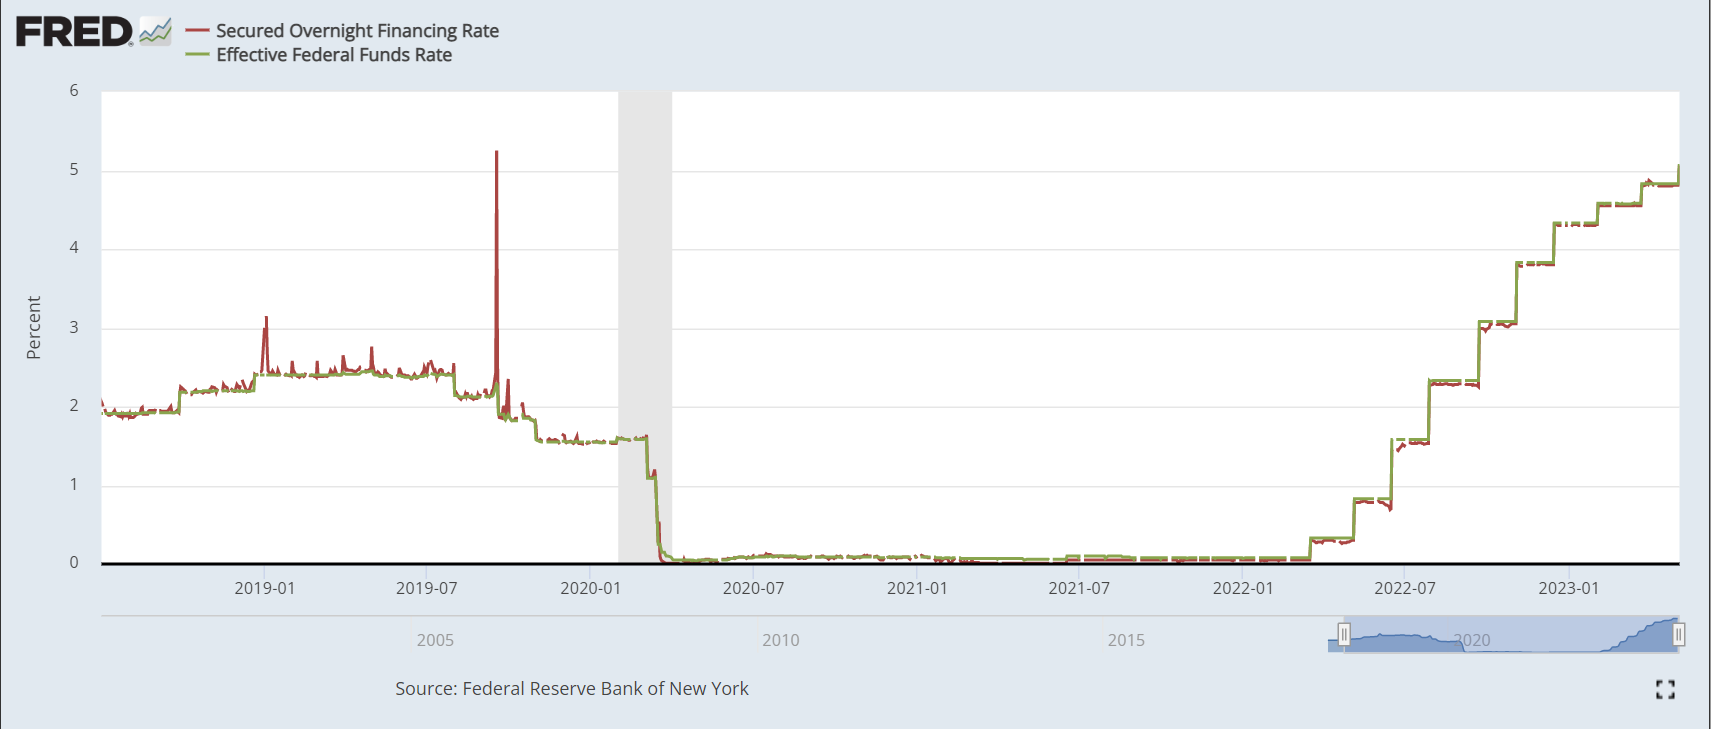
\includegraphics[height = 7cm, width=15cm]{figures/SOFR/SOFR_EFFR.PNG}
    \caption{SOFR and EFFR}
    \label{fig: SOFR_EFFR}
\end{figure}


As mentioned earlier, we have that SOFR is backwards-looking and cannot give any indications beyond 24 hours. However, the CME Group publishes daily a set of forward-looking interest rate estimates called CME Term SOFR Reference Rates Benchmarks. 
They have the following tenors: 1M, 3M, 6M and 12M. 


\begin{figure}[htp]
    \centering
    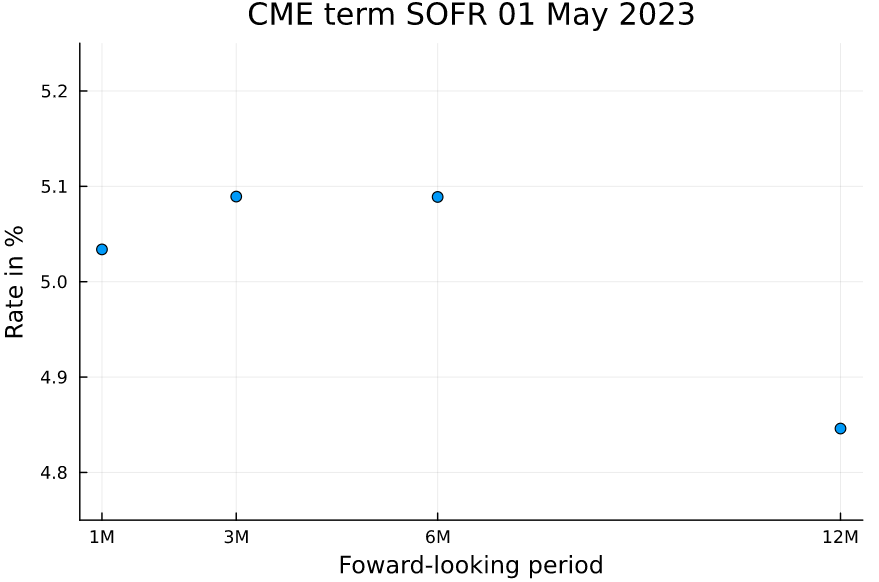
\includegraphics[width=12cm]{figures/SOFR/CME_term_SOFR.PNG}
    \caption{CME term SOFR }
    \label{fig: CME_term_SOFR}
\end{figure}



\begin{comment}
The calculation method can be found in\cite{CMEGroup}. For modelling SOFR dynamics \cite{gellert2021short} can be consulted.  
\\~\\ 
\end{comment}

\newpage 

They use SOFR futures for calculating the term rates. The calculation method can be found at \cite{CMEGroup}. Some of the reasons why futures were chosen were because of their liquidity. This represents the market's view on the rate; furthermore, this does not require expert judgment or a survey of market participants.  

\begin{figure}[htp]
    \centering
    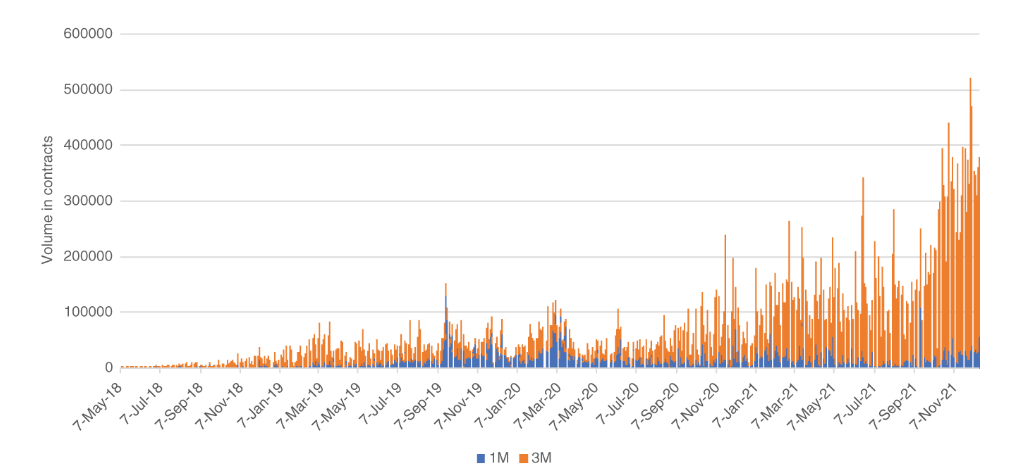
\includegraphics[width=14cm]{figures/SOFR/SOFR_future_volume.PNG}
    \caption{Daily volume of SOFR futures, source: \cite{huggins2022sofr} }
    \label{fig: Volume_SOFR_futures}
\end{figure}

We see that there are some significant differences between the volumes. This is further discussed in \cite{huggins2022sofr}, where some of the explanation could be of the calculation methods for SOFR futures, i.e. arithmetic and geometric. However, it is also mentioned that there may be a boost in demand for 1M-SOFR futures when LIBOR is fully phased out. 









\newpage 
\begin{comment}
\begin{figure}[htp]
    \centering
    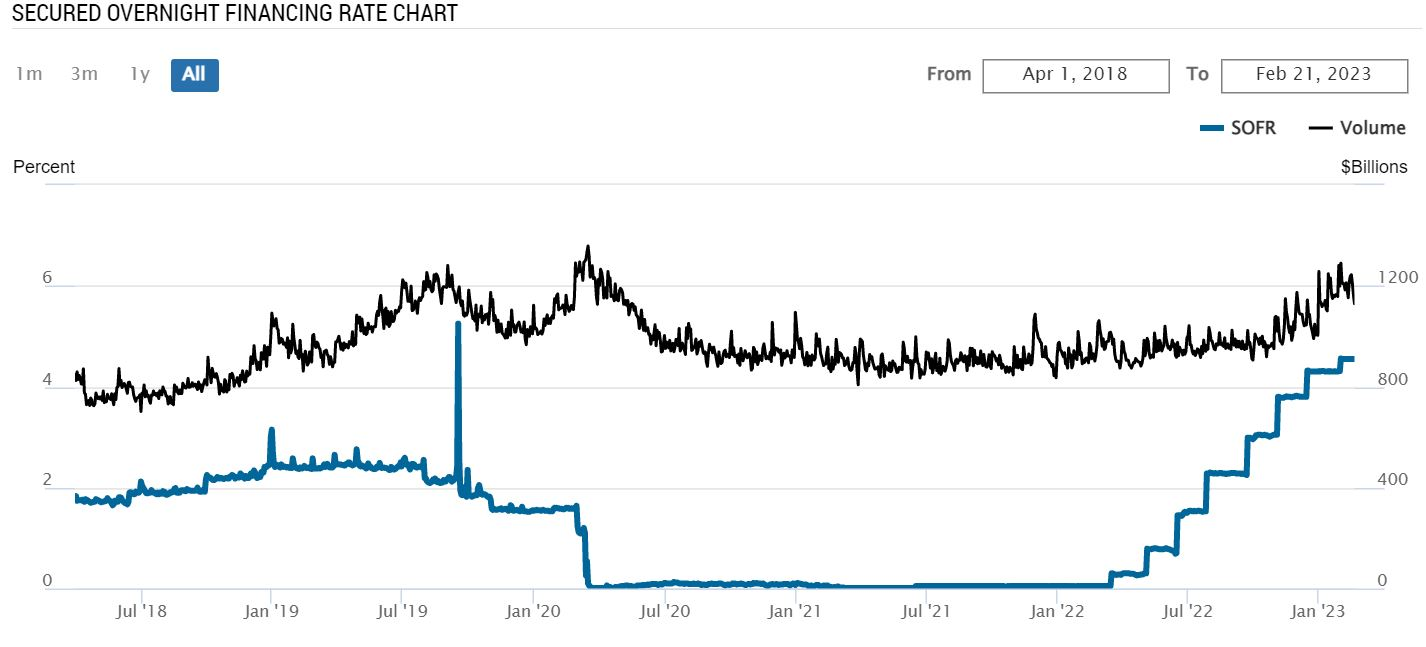
\includegraphics[height = 7cm, width=14cm]{figures/SOFR/overnight_SOFR_Volume.JPG}
    \caption{Overnight SOFR rates. Source: \cite{NewYorkFedSOFR}}
    \label{fig: Overnight_SOFR_rates}
\end{figure}



This Figure shows the overnight SOFR rates from April 1, 2018, until February 21, 2023, with corresponding traded volumes.
\\~\\
We see that there was a spike in September 2019. This was related to quarterly corporate tax payments due September 16. This led to a demand-supply mismatch  \cite{FederalReserve2019}
\\~\\ 
We also see the effect of the pandemic with falling rates around March 2020, until now, the rising rates. 
\end{comment}

\newpage 

\section{SOFR futures}
Let $(\Omega, \F, (\F_{t})_{t\geq 0}, Q)$ denote our probability space, and let $Q$ be the risk-neutral probability measure defined via  the money market account $B(t)$ as numeraire. 
\\~\\
\begin{definition}[\textbf{Futures contract \cite{björk2019arbitrage}}]
A futures contract on $X$ with delivery $T$, is a financial asset with following properties: 
\begin{enumerate}[leftmargin =*]
    \item For all $t$ with $0\leq t \leq T$, there exists in the market a quoted object $f(t,T;X)$ known as the futures price of $X$ at time $t$, with delivery $T$. 
    \item At time $T$ of delivery, the holder of the contract pays: $f(T,T;X)$ and receives the claim $X$.
    \item During an arbitrary interval $(s,t]$, the holder of the contract receives: 
    \[
    f(t,T;X) - f(s,T;X)
    \]
\end{enumerate}
\end{definition}

In typical futures contracts, the underlying asset  
$X$ could be oil barrels, corn, cattle etc. In our situation, the underlying asset is an interest rate. The typical settlement is a cash settlement. 
\\~\\ 
\textbf{Some reasons to enter a futures contract:}
\begin{itemize}
    \item Speculation: By trading futures, one can make money by differences in quotes.  
    \item Hedging: One could hedge against higher/lower interest rates. For instance, someone paying a floating rate might buy futures to lock in a future interest rate. 
\end{itemize}



We will be interested in SOFR futures, and such futures can be found at CME (Chicago Mercantile Exchange) \nomenclature{CME}{Chicago Mercantile Exchange}. CME uses the following convention for quoting interest rate futures: 
\[
100 - R
\]
Here $R$ will represent the implied SOFR rate. Let's say we observe a 3M-SOFR futures today (March 23) with settlement Jun 23, quoted at $96.6$. This would mean that the implied $3M$-SOFR rate (annualized) over the period March 23 - June 23 would be: 
\[
(100-96.6)\% = 3.4\% 
\] 
Further specifications on how CME quotes 3M-SOFR futures can be found in  \cite{cmegroup-sofr-futures}. 

\newpage 

When dealing with SOFR futures, one distinguishes between 1-month- and 3-month futures, as they are not based upon the same calculation methodology:

\begin{definition}[\textbf{SOFR 1-month arithmetic average \cite{Skov_2020}}]
The 1-month \nomenclature{1M}{1-month}
SOFR arithmetic average of the daily reference rate observed over the period $[S,T]$ is defined as: 
\[
R^{1M}(S,T) = \frac{1}{N}\sum_{i=1}^{N}R_{d_{i}}(T_{i})
\]
Where:
\begin{itemize}[leftmargin=*]
    \item $N$: total number of days in the month
    \item $S\leq T_{1} \leq \dots \leq T_{N} \leq T$ 
\end{itemize}
\end{definition}



\begin{definition}[\textbf{SOFR 3-month geometric average}]
The 3-month \nomenclature{3M}{3-months}
SOFR geometric average of the daily reference rate observed over the period $[S,T]$ is defined as: 
\[
R^{3M}(S,T) = \frac{1}{T-S}\left(
\prod_{i=1}^{N}(1+d_{i}R_{d_{i}}(T_{i})) - 1
\right)
\]
\end{definition}



As futures contracts are free to enter, we get that: 
\begin{align*}
\E_{Q}\left[
R^{\ell M}(S,T) - f^{\ell M}(t,S,T)\bigg{|}\F_{t}
\right] = 0, \;\; \ell = 1,3   
\end{align*}

Furthermore, one uses the following convention: 
\begin{align*}
R^{1M}(S,T) \approx  \frac{1}{T-S}\int_{S}^{T}r(s)ds 
\;\;\text{and}\;\;
R^{3M}(S,T) \approx  \frac{1}{T-S}\left(e^{\int_{S}^{T}r(s)ds} -1\right) 
\end{align*}

This gives rise to the following definitions:

\begin{definition}[\textbf{1-month SOFR futures \cite{Skov_2020}}]
\label{def: 1M_SOFR_futures}
\nomenclature{$f^{1M}(t,S,T)$}{1-month SOFR futures}
We denote the time $t$ rate of the 1-month futures starting to accrue at time $S$ and with settlement on time $T$ as:
\begin{align*}
f^{1M}(t,S,T) &= \frac{1}{T-S}\E_{Q}\left[
\int_{S}^{T}r(s)ds\bigg{|}\F_{t}
\right]    
\end{align*}
\end{definition} 

\begin{definition}[\textbf{3-month SOFR futures \cite{Skov_2020}}]
\label{def: 3M_SOFR_futures}
\nomenclature{$f^{3M}(t,S,T)$}{3-month SOFR futures}
We denote the time $t$ rate of the 3-month futures starting to accrue at time $S$ and with settlement on time $T$ as:  
\begin{align*}
f^{3M}(t,S,T) &= \frac{1}{T-S}\left(
\E_{Q}\left[e^{\int_{S}^{T}r(s)ds}\bigg{|}\F_{t}\right] - 1
\right)    
\end{align*}
\end{definition} 

\newpage 

\begin{proposition}[\textbf{Vasicek dynamics of 1M/3M-SOFR futures, [Exercise STK4530, Autumn 2021]}]
Assume that the short rate has the following dynamics: 
\begin{align*}
dr(t) &= \alpha[m-r(t)]dt + \sigma dW^{Q}(t)    
\end{align*}

Then the dynamics of $f^{1M}(t,S,T)$ is given by:
\begin{align*}
df^{1M}(t,S,T) &= \frac{1}{T-S}B(t,S,T)\sigma dW^{Q}(t)
\end{align*}

and the dynamics of $f^{3M}(t,S,T)$ is given by: 
\begin{align*}
df^{3M}(t,S,T) &= \left(
f^{3M}(t,S,T) +\frac{1}{T-S}
\right)B(t,S,T)\sigma dW^{Q}(t)
\end{align*}

Where: 
\begin{align*}
B(t,S,T) &= \frac{1}{\alpha}\left[
e^{-\alpha(S-t)}-e^{-\alpha(T-t)}
\right]    
\end{align*}
\end{proposition}


\begin{proof}

From Proposition \ref{prop: Vasicek_ATS}, we have that: 
\begin{align*}
r(s) &= e^{-\alpha(s-t)}r(t) + m[1-e^{-\alpha(s-t)}] + \sigma \int_{t}^{s}e^{-\alpha(s-u)}dW^{Q}(u)
\end{align*}

Now: $f^{1M}(t,S,T) = \frac{1}{T-S}\E_{Q}\left[\int_{S}^{T}r(s)ds|\F_{t} \right]$:  
\begin{align*}
\E_{Q}\left[
r(s)|\F_{t}
\right]
&= 
r(t)e^{-\alpha(s-t)} + m\left(1-e^{-\alpha(s-t)}\right) \\ 
&\Downarrow \\ 
f^{1M}(t,S,T)
&= 
\frac{e^{-\alpha S}- e^{-\alpha T}}{\alpha(T-S)}[r(t)-m]e^{\alpha t}
+ m 
\end{align*}

Giving rise to the following dynamics: 
\begin{align*}
df^{1M}(t,S,T) 
&= 
\frac{e^{-\alpha S}- e^{-\alpha T}}
{\alpha(T-S)}
d\left[
(r(t)-m)e^{\alpha t}
\right]
\end{align*}

Let's work with the differential part first: 
\begin{align*}
d[(r(t)-m)e^{\alpha t}] &= d[r(t)e^{\alpha t}] - md(e^{\alpha t}) \\
&= \alpha me^{\alpha t}dt + \sigma e^{\alpha t}dW^{Q}(t) - \alpha me^{\alpha t}dt \\ 
&= 
\sigma e^{\alpha t}dW^{Q}(t)
\end{align*}

Thus: 
\begin{align*}
df^{1M}(t,S,T) 
&= 
\frac{e^{-\alpha S}- e^{-\alpha T}}
{\alpha(T-S)}\sigma e^{\alpha t}dW^{Q}(t) \\ 
&= \frac{1}{T-S}B(t,S,T)\sigma dW^{Q}(t)
\end{align*}

\newpage 
Now for $f^{3M}(t,S,T)$ we must study $\int_{S}^{T}r(s)ds$:  
\\~\\
We have the following timeline:

\begin{tikzpicture}[snake=zigzag, line before snake = 5mm, line after snake = 5mm]
    % draw horizontal line   
    \draw (0,0) -- (4,0);
    
    % draw vertical lines
    \foreach \x in {0,1,2,3, 4}
      \draw (\x cm,3pt) -- (\x cm,-3pt);

    % draw nodes
    \draw (0,0) node[below=3pt] {$ t $} node[above=3pt] {$   $};
    \draw (1,0) node[below=3pt] {$ S $} node[above=3pt] {$  $};
    \draw (2,0) node[below=3pt] {$ u $} node[above=3pt] {$  $};
    \draw (3,0) node[below=3pt] {$ s $} node[above=3pt] {$  $};
    \draw (4,0) node[below=3pt] {$ T $} node[above=3pt] {$  $};
  \end{tikzpicture}

namely $t\leq S \leq u \leq s \leq T$, this gives us: 
\begin{align*}
\int_{S}^{T}r(s)ds &= \frac{r(t)}{\alpha}\left[
e^{-\alpha(S-t)} - e^{-\alpha(T-t)}
\right]   
+ m(T-S) - \frac{m}{\alpha}\left[
e^{-\alpha(S-t)} - e^{-\alpha(T-t)}
\right] \\ 
&+ 
\sigma 
\underbrace{
\int_{S}^{T}\int_{t}^{s}e^{-\alpha(s-u)}dW^{Q}(u)ds
}_{=(*)}
\end{align*}

Now by additivity of the integral, we see that: 
\begin{align*}
\int_{t}^{s} = \int_{t}^{S} + \int_{S}^{s}    
\end{align*}

This leaves us with: 
\begin{align*}
(*) &= 
\int_{S}^{T}\left(
\int_{t}^{S}e^{-\alpha(s-u)}dW^{Q}(u) + \int_{s}^{S}e^{-\alpha(s-u)}dW^{Q}(u)
\right)ds \\ 
&= 
\underbrace{
\int_{S}^{T}\int_{t}^{S}e^{-\alpha(s-u)}dW^{Q}(u)ds 
}_{=(1)}
+ 
\underbrace{
\int_{S}^{T}\int_{S}^{s}e^{-\alpha(s-u)}dW^{Q}(u)ds
}_{= (2)}
\end{align*}

By Stochastic Fubini, we get: 
\begin{align*}
(1) &= \int_{S}^{T}\int_{t}^{S}e^{-\alpha(s-u)}dW^{Q}(u)ds 
= \int_{t}^{S}\int_{S}^{T}e^{-\alpha(s-u)}dsdW^{Q}(u) 
= (1)'
\end{align*}


\begin{tikzpicture}[snake=zigzag, line before snake = 5mm, line after snake = 5mm]
    % draw horizontal line   
    \draw (0,0) -- (4,0);
    
    % draw vertical lines
    \foreach \x in {0,2,4}
      \draw (\x cm,3pt) -- (\x cm,-3pt);

    % draw nodes
    \draw (0,0) node[below=3pt] {$ S $} node[above=3pt] {$   $};
    \draw (1,0) node[below=3pt] {$  $} node[above=3pt] {$  $};
    \draw (2,0) node[below=3pt] {$ u $} node[above=3pt] {$  $};
    \draw (3,0) node[below=3pt] {$  $} node[above=3pt] {$  $};
    \draw (4,0) node[below=3pt] {$ s $} node[above=3pt] {$  $};
  \end{tikzpicture}


\begin{align*}
\begin{cases}
 S \leq s \leq T \\ 
 S \leq u \leq s
\end{cases}
&\iff
\begin{cases}
 u \leq s \leq T \\ 
 S \leq u \leq T
\end{cases}
\end{align*}

Now this leaves us with the following: 
\begin{align*}
(2) =\int_{S}^{T}\int_{S}^{s}e^{-\alpha(s-u)}dW^{Q}(u)ds 
=
\int_{S}^{T}\int_{u}^{T}e^{-\alpha(s-u)}dsdW^{Q}(u) = (2)'
\end{align*}

We now calculate the inner integral in $(1)'$ and $(2)'$ respectively: 
\begin{align*}
\int_{S}^{T}e^{-\alpha(s-u)}ds &= \frac{1}{\alpha}\left[
e^{\alpha(S-u)}-e^{-\alpha(T-u)}
\right] \\ 
\int_{u}^{T}e^{-\alpha(s-u)}ds &= \frac{1}{\alpha}\left[
1 -e^{-\alpha(T-u)}
\right]
\end{align*}

We can then define: 
\begin{align*}
\Sigma(u,t,S,T) &= 
    \begin{cases}
      e^{\alpha(S-u)}-e^{-\alpha(T-u)},  & u \in [t,S)\\
      1 -e^{-\alpha(T-u)}, & u\in [S,T]
    \end{cases}
\end{align*}

We are thus left with: 
\begin{align}
\label{eq: Vasicek_closed_expr_3M_SOFR}
\int_{S}^{T}r(s)ds &= \frac{r(t)}{\alpha}\left[
e^{-\alpha(S-t)} - e^{-\alpha(T-t)}
\right]   
+ m(T-S) - \frac{m}{\alpha}\left[
e^{-\alpha(S-t)} - e^{-\alpha(T-t)}
\right] \nonumber \\
&+ \frac{\sigma}{\alpha}\int_{t}^{T}\Sigma(u,t,S,T)dW^{Q}(u)\nonumber \\ 
&= 
\left(
\frac{r(t)-m}{\alpha}
\right)
\left[
e^{-\alpha(S-t)} - e^{-\alpha(T-t)}
\right]
+ m(T-S) 
+ 
\underbrace{
\frac{\sigma}{\alpha}\int_{t}^{T}\Sigma(u,t,S,T)dW^{Q}(u)
}_{\F_{t}-\text{independent}}
\end{align}


As the last part is $\F_{t}$-independent,we get: 
\begin{align*}
\E_{Q}\left[
\exp\left(
\int_{S}^{T}r(s)ds
\right)\bigg{|}\F_{t}
\right] 
&= 
\exp\left[
\left(
\frac{r(t)-m}{\alpha}
\right)
\left[
e^{-\alpha(S-t) - e^{-\alpha(T-t)}}
\right]
+ m(T-S) 
\right] \\
&\times  
\E_{Q}\left[
\exp\left(
\frac{\sigma}{\alpha}\int_{t}^{T}\Sigma(u,t,S,T)dW^{Q}(u)
\right)
\right]
\end{align*}

Since $\Sigma$ is deterministic, we have that: 
\begin{align*}
\E_{Q}\left[
\exp\left(
\frac{\sigma}{\alpha}\int_{t}^{T}\Sigma(u,t,S,T)dW^{Q}(u)
\right)
\right]
&= 
\exp\left(
\frac{1}{2}\frac{\sigma^{2}}{\alpha^{2}}\int_{t}^{T}\Sigma^{2}(u,t,S,T)du
\right)
\end{align*}

This leaves us with the following expression:
\begin{align}
\label{eq: a_hat_3M_SOFR}
 \E_{Q}\left[
\exp\left(
\int_{S}^{T}r(s)ds
\right)\bigg{|}\F_{t}
\right] 
&= 
\exp\left(
A(t,S,T) + B(t,S,T)r(t)
\right):= g(t,r(t))
\end{align}

where: 
\begin{align*}
A(t,S,T) &= m(T-S) - \frac{m}{\alpha}\left[
e^{-\alpha(S-t)} - e^{-\alpha(T-t)}
\right] + \frac{1}{2}\frac{\sigma^{2}}{\alpha^{2}}\int_{t}^{T}\Sigma^{2}(u,t,S,T)du \\
B(t,S,T) &= \frac{1}{\alpha}\left[
e^{-\alpha(S-t)} - e^{-\alpha(T-t)}
\right]
\end{align*}

This means that we have: 
\begin{align}
\label{eq: Vasicek_3M_SOFR_closed_formula}
f^{3M}(t,S,T) &= \frac{1}{T-S}\left[
g(t,r(t)) - 1
\right]    
\end{align}

We note that $\E_{Q}\left[
\exp\left(
\int_{S}^{T}r(s)ds
\right)\bigg{|}\F_{t}
\right]$ is a $Q$-martingale, thus from the Martingale Representation Theorem \ref{thm: Martingale_rep_thm}, we can neglect the dt-terms of $g(t,r(t))$:
\\~\\
We apply Ito's Formula as $g(t,x) \in C^{1,2}([0,\infty]\times \R)$, giving us: 
\begin{align*}
\partial_{t}g(t,x) &= 0, \;\; \partial_{x}g(t,x) = g(t,x)B(t,S,T), \;\; 
\partial_{xx}g(t,x) = g(t,x)B^{2}(t,S,T) \\ 
dr(t)^{2} &= \sigma^{2}dt \\ 
&\Downarrow \\ 
dg(t,r(t)) &= B(t,S,T)g(t,r(t))\sigma dW^{Q}(t)
\end{align*}

\newpage 

This gives the following dynamics for $f^{3M}(t,S,T)$:
\begin{align*}
df^{3M}(t,S,T) &= \frac{1}{T-S}dg(t,r(t)) \\ 
&= \frac{1}{T-S}B(t,S,T)\exp\left(A(t,S,T) + B(t,S,T)r(t)\right)\sigma dW^{Q}(t)\\ 
&= 
\frac{1}{T-S}B(t,S,T)\left[
(T-S)f^{3M}(t,S,T) +1
\right]\sigma dW^{Q}(t) \\ 
&= 
\left(
f^{3M}(t,S,T) + \frac{1}{T-S}
\right)B(t,S,T)\sigma dW^{Q}(t)
\end{align*}
\end{proof}

To get a bit better grasp of the SOFR futures rates $f^{1M}$ and $f^{3M}$, we include a graph of possible $Q$-dynamics: 

\begin{figure}[htp]
    \centering
    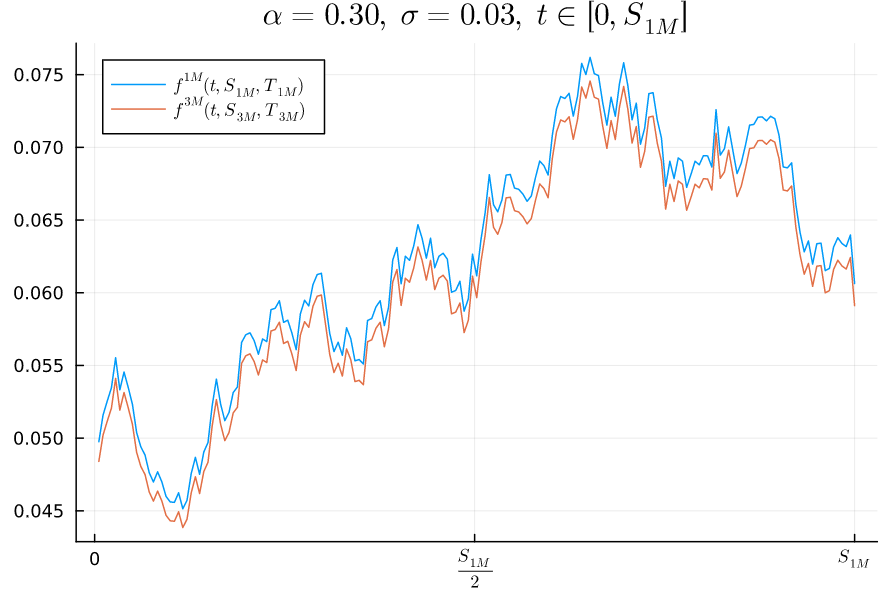
\includegraphics[width=12cm]{figures/SOFR/1M_3M_futures_dynamics.PNG}
    \caption{Realization of $f^{1M}(t,S_{1M}, T_{1M})$ and $f^{3M}(t,S_{3M}, T_{3M})$ for $t\in [0,S_{1M}]$}
    \label{fig: 1M_3M_futures_dynamics}
\end{figure}


Here we have assumed that the quotes for 1M and 3M futures differ. We took: 
\begin{align*}
f^{1M}(0, S_{1M}, T_{1M}) &= (100-95.025)\cdot\frac{1}{100} \approx 0.0498 \\ 
f^{3M}(0, S_{3M}, T_{3M}) &= (100-95.160)\cdot\frac{1}{100} \approx 0.0484
\end{align*}
Furthermore, we have $S_{1M} = S_{3M} = 6$ months, and $f^{1M}, f^{3M}$ are generated by the same Brownian motion. 


\newpage 

\section{Interest rate swap with SOFR-futures as floating}


\begin{proposition}
The fixed swap rate $\kappa_{t}^{\ell M-SOFR}$ in a swap with 1M/3M-SOFR as floating is given by:  
\begin{align*}
 \kappa_{t}^{\ell M-SOFR} &= 
 \frac{
 \sum_{i=1}^{n}P(t,T_{i})f^{\ell M}(t,T_{i-1}, T_{i})
 }{
 \sum_{i=1}^{n}P(t,T_{i})
 }, \;\; \ell = 1,3
\end{align*}
\end{proposition}

\begin{proof}
    
In this swap, we have the following specification, at time $T_{i}$:
\begin{itemize}[leftmargin=*]
    \item Pay $\kappa_{t}^{\ell M-SOFR}\delta N$ (-)
    \item Receive $f^{\ell M}(t,T_{i-1}, T_{i})\delta N$, \; $\ell=1,3$ (+)
\end{itemize} 

\textbf{Cash flow at time $T_{i}$}:
\begin{align*}
f^{\ell M}(t, T_{i-1}, T_{i})\delta N - \kappa_{t}^{\ell M-SOFR}\delta N =
[f^{\ell M}(t,T_{i-1}, T_{i}) -\kappa_{t}^{\ell M-SOFR}]\delta N, \;\; \ell =1,3
\end{align*}

\textbf{Time $t$-value for $t\leq T_{0}$ at time $T_{i}$}: 
\begin{align*}
P(t,T_{i})[f^{\ell M}(t,T_{i-1}, T_{i}) - \kappa_{t}^{SOFR}]\delta N,\;\; \ell =1,3
\end{align*}

\textbf{Total payer cash flow:}
\begin{align*}
\mathcal{C}_{P}^{\ell M-SOFR}(t) &= 
\delta N \sum_{i=1}^{n}P(t,T_{i})[f^{\ell M}(t,T_{i-1}, T_{i}) - \kappa_{t}^{\ell M-SOFR}], \;\; \ell =1,3
\end{align*} 

$\kappa_{t}^{\ell M-SOFR}$ should be chosen such that: 
\begin{align*}
\E_{Q}[\mathcal{C}_{P}^{\ell M-SOFR}(t)|\F_{t}] = 0    
\end{align*}

Thus: 
\begin{align*}
\sum_{i=1}^{n}P(t,T_{i})f^{\ell M}(t,T_{i-1}, T_{i}) &= \sum_{i=1}^{n}P(t,T_{i})\kappa_{t}^{\ell M-SOFR} \\ 
&\Downarrow \\ 
\kappa_{t}^{\ell M-SOFR} &= \frac{
\sum_{i=1}^{n}P(t,T_{i})f^{\ell M}(t,T_{i-1}, T_{i})
}{
\sum_{i=1}^{n}P(t,T_{i})
}
\end{align*}
\end{proof}

\newpage 

Let us consider the case where we look at $\ell=3$, $n=3$, and $\delta = \frac{3}{12}$. For simplicity, we choose the Vasicek model as this gives an explicit formula for $f^{3M}(t,S,T)$ as described in Equation \ref{eq: Vasicek_3M_SOFR_closed_formula}.

\begin{figure}[htp]
    \centering
    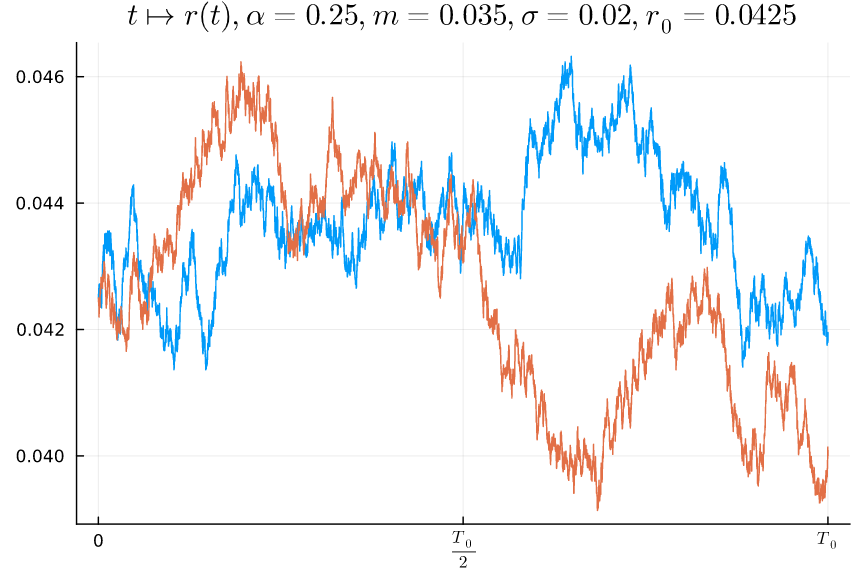
\includegraphics[width=12cm]{figures/SOFR/Vasicek_realizations.PNG}
    \caption{Realizations of $t \mapsto r(t), t \in [0,T_{0}]$}
    \label{fig: Vasicek_paths}
\end{figure}

Here we see two realizations of $[0,T_{0}] \ni t \mapsto r(t)$. In the graph below, we see the effect of the time horizon and the starting point for the fixed rate $\kappa_{t}^{3M-SOFR}$:


\begin{figure}[htp]
    \centering
    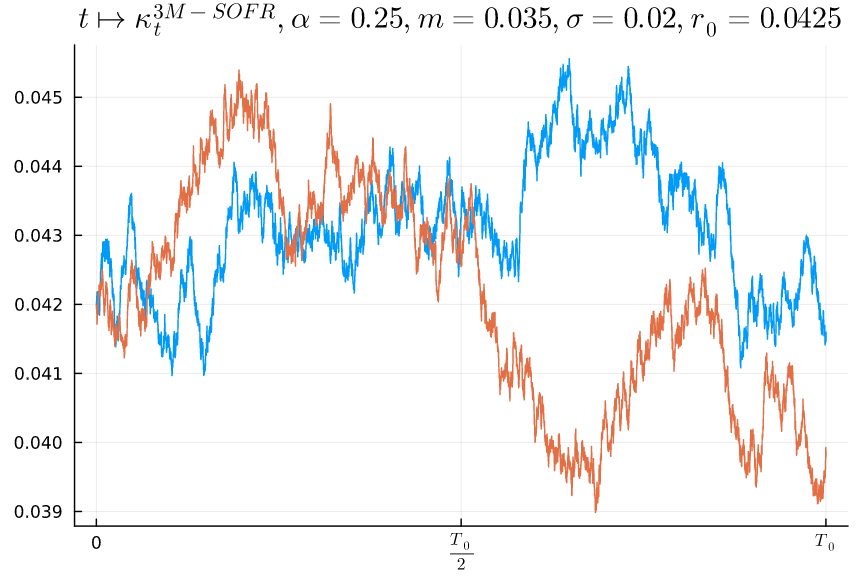
\includegraphics[width=12cm]{figures/SOFR/3M_SOFR_swap_rate_Vasicek.PNG}
    \caption{Realizations of $t \mapsto \kappa_{t}^{3M-SOFR}, t \in [0,T_{0}]$}
    \label{fig: 3M_SOFR_swap_rate}
\end{figure}

Here we took two realizations of $[0,T_{0}] \ni t \mapsto \kappa_{t}^{3M-SOFR}$. For $t=0$, we got: 
\begin{align*}
\kappa_{0}^{3M-SOFR} &= 
\frac{
\sum_{i=1}^{3}P(0,T_{i})f^{3M}(0,T_{i-1}, T_{i})
}{
\sum_{i=1}^{3}P(0,T_{i})
}
= 
0.042
\end{align*}





\newpage 

\section{Options on SOFR futures}

Consider a call option on SOFR futures, with exercise time $\tau \leq S \leq T$ and strike $\kappa$, the price at time $t \leq \tau$ for $\ell =1,3$ is given by:
\begin{align*}
C^{\ell M}(t,\tau) :&= \E_{Q}\left[
\frac{B(t)}{B(\tau)}\left(
f^{\ell M}(\tau,S,T) - \kappa
\right)^{+}
\bigg{|}\F_{t}
\right]  
&\stackrel{\text{Prop \ref{prop: general_option_price}}}{=} 
P(t,\tau)\E_{Q^{\tau}}\left[
\left(f^{\ell M}(\tau,S,T) - \kappa
\right)^{+}
\bigg{|}\F_{t}
\right]
\end{align*} 

Here we use the convention that $(x)^{+} = \max(x,0)$. From Theorem \ref{thm: arbitrage_condition_Q} p \pageref{thm: arbitrage_condition_Q}, we have: 
\begin{align*}
\frac{dQ^{\tau}}{dQ}\bigg{|}_{\F_{t}} &= \mathcal{E}_{t}(v(\cdot, \tau)\bullet W^{Q})
\end{align*} 

Assuming Novikov's condition holds, i.e: $\E_{Q}\left[e^{\frac{1}{2}\int_{0}^{T}\norm{v(s,\tau)}^{2}ds}\right] < \infty$ we get from Girsanov's theorem, that
\begin{align*}
dW^{\tau}(t) &= dW^{Q}(t) - v(t,\tau)dt    
\end{align*}
defines a $Q^{\tau}$-Brownian motion. 
\\~\\ 
\begin{proposition}[\textbf{1M-SOFR futures Caplet [Lecture STK4530]}]
Consider a call option on the 1M-SOFR futures with exercise time $\tau \leq T$ and strike $\kappa$. Let 
\[
df^{1M}(t,S,T) = \Sigma^{1M}(t,S,T)dW^{Q}(t)  
\]
Where $\Sigma^{1M}(t,S,T)$ is assumed to be a deterministic and bounded function. The price at time $t\leq \tau$ is given by: 
\begin{align*}
C^{1M}(t,\tau) &= 
P(t,\tau)\sqrt{
\int_{t}^{\tau}\Sigma^{1M}(u,S,T)^{2}du
}\left[
d\Phi(d) + \varphi(d)
\right]
\end{align*}
Where: 
\begin{align*}
d &= 
\frac{
f^{1M}(t,S,T) + \int_{t}^{\tau}\Sigma^{1M}(u,S,T)v(u,\tau)du - \kappa
}{
\sqrt{
\int_{t}^{\tau}\Sigma^{1M}(u,S,T)^{2}du
}
}
\end{align*}
And $\Phi, \varphi$ represents the cumulative and density function of a standard-normal distribution respectively. 
\end{proposition}

\begin{proof}
The $Q^{\tau}$-dynamics are given by: 
\begin{align*}
df^{1M}(t,S,T) &= 
\Sigma^{1M}(t,S,T)v(t,\tau)dt + \Sigma^{1M}(t,S,T)dW^{\tau}(t)\\ 
&\Downarrow \\ 
f^{1M}(\tau,S,T) &= 
\underbrace{f^{1M}(t,S,T)}_{x} + 
\underbrace{\int_{t}^{\tau}\Sigma^{1M}(u,S,T)v(u,\tau)du}_{m} +  
\int_{t}^{\tau}\Sigma^{1M}(u,S,T)dW^{\tau}(u)
\end{align*}    

Let 
\[
b^{2} = \int_{t}^{\tau}\Sigma^{1M}(u,S,T)^{2}du
\]

We are then left with the following: 
\begin{align*}
\E_{Q^{\tau}}\left[
(f^{1M}(\tau, S,T)-\kappa)^{+}\bigg{|}\F_{t}
\right]    
= 
\E\left[
(x+m+bZ-\kappa)^{+}
\right]\bigg{|}_{x = f^{1M}(t,S,T)}
\end{align*}

where $Z \sim \mathcal{N}(0,1)$, this yields: 

\begin{align*}
\E\left[
(x+m+bZ-\kappa)^{+}
\right]\bigg{|}_{x = f^{1M}(t,S,T)} 
&= 
\int_{\R}(x+m+bz-\kappa)^{+}\varphi(z)dz 
\end{align*}

Furthermore: 
\begin{align*}
x + m + bz - \kappa \geq 0 \iff z \geq \frac{\kappa-x-m}{b}:= d'    
\end{align*}

This yields: 
\begin{align*}
\int_{\R}(x+m+bz-\kappa)^{+}\varphi(z)dz  
&= 
\underbrace{
(x+m-\kappa)\int_{d'}^{\infty}\varphi(z)dz
+ b\int_{d'}^{\infty}z\varphi(z)dz
}_{(A)}
\end{align*}

By symmetry of the normal distribution we have: $P(Z > d') = P(Z \leq -d')$, 
where we define: 
\[
d := -d' = \frac{x+m-\kappa}{b}
\]
furthermore $z\varphi(z) = - \varphi'(z)$, thus:

\begin{align*}
\int_{d'}^{\infty}z\varphi(z)dz
&= 
-\int_{d'}^{\infty}\varphi'(z)dz 
= 
-(\varphi(\infty) - \varphi(d'))
= \varphi(d') = \varphi(d)
\end{align*}

Leaving us with:
\begin{align*}
(A) &= (x+m-\kappa)\Phi(d) + b\varphi(d) \\ 
&= b[d\Phi(d) + \varphi(d)]
\end{align*}
Now from Proposition \ref{prop: general_option_price} p.\pageref{prop: general_option_price}, we get: 
\begin{align*}
C^{1M}(t,\tau) &= P(t,\tau)\E_{Q^{\tau}}\left[
(f^{1M}(\tau, S,T)-\kappa)^{+}\bigg{|}\F_{t}
\right] \\ 
&= 
P(t,\tau)\sqrt{
\int_{t}^{\tau}\Sigma^{1M}(u,S,T)^{2}du
}\left[
d\Phi(d) + \varphi(d)
\right]
\end{align*}
\end{proof}


\newpage 

\section{Hedging with SOFR-futures}
For SOFR futures, we have two pricing approaches: arithmetic (1M) and geometric (3M). In this section, we will look at some relationships between them.


\subsection{Hedging 3-month arithmetic with 3-month geometric}
Consider the case where we want to hedge:

\begin{align}
\label{eq: X_3MA(S,T)}
X^{3M_{A}}(S,T) = \frac{1}{T-S}\int_{S}^{T}r_{u}du    
\end{align}

We want to hedge an arithmetic interest rate over the 3M period $[S,T]$. The only available product for hedging a 3M period in the market is the 3M futures contract $f^{3M}(t,S,T)$. 

\begin{proposition}
\label{prop: optimal_hedge_arithmetic_3M_geometric}
\begin{align*}
\argmin\limits_{a_{t} \in \R}\E_{Q}\left[
\left(
X^{3M_{A}}(S,T)-a_{t}f^{3M}(t,S,T)
\right)^{2}
\bigg{|}\F_{t}
\right] 
= \frac{
\int_{S}^{T}\E_{Q}[r(u)|\F_{t}]du
}{
(T-S)f^{3M}(t,S,T)
}
\end{align*}

Meaning that the optimal weighting $\hat{a}_{t}^{3M}$ in 3M-SOFR futures will be: 

\begin{align*}
\hat{a}_{t}^{3M} &= \frac{
\int_{S}^{T}\E_{Q}[r(u)|\F_{t}]du
}{
(T-S)f^{3M}(t,S,T)
}   
\end{align*}
\end{proposition}

\begin{proof}
    
We have that the 3M-SOFR futures $f^{3M}(t,S,T)$ is based upon a geometric average, giving us the following hedge:

\begin{align*}
\argmin\limits_{a_{t} \in \R}\E_{Q}\left[
\left(
X^{3M_{A}}(S,T)-a_{t}f^{3M}(t,S,T)
\right)^{2}
\bigg{|}\F_{t}
\right]
\end{align*}

Now, fix $t$ and denote: 
\begin{align*}
G(a_{t}) :=\E_{Q}\left[
\left(X^{3M_{A}}(S,T)-a_{t}f^{3M}(t,S,T)
\right)^{2}
\bigg{|}\F_{t}
\right]    
\end{align*} 

Expanding the square yields:
\begin{align*}
G(a_{t}) &= \E_{Q}\left[(X^{3M_{A}}(S,T))^{2}|\F_{t}\right] -2a_{t}f^{3M}(t,S,T)\E_{Q}\left[X^{3M_{A}}(S,T)\bigg{|}\F_{t}\right] +
a_{t}^{2}[f^{3M}(t,S,T)]^{2}
\end{align*}
Taking the derivative w.r.t. $a_{t}$ yields: 
\begin{align*}
\frac{d}{da_{t}}G(a_{t}) &= -2f^{3M}(t,S,T)
\E_{Q}\left[X^{3M_{A}}(S,T)\bigg{|}\F_{t}\right] + 2a_{t}[f^{3M}(t,S,T)]^{2}  
\end{align*} 

\newpage 

Since: 
\begin{align*}
\frac{d^{2}}{da_{t}^{2}}G(a_{t}) = 2[f^{3M}(t,S,T)]^{2} > 0    
\end{align*}

We have that the minimum is obtained by setting the derivative equal to zero, i.e. 
\begin{align*}
\frac{d}{da_{t}}G(a_{t}) = 0    
\end{align*}

Now: 
\begin{align*}
\frac{d}{da_{t}}G(a_{t}) &= 0 \\
&\Updownarrow \\ 
a_{t} &= \frac{
\E_{Q}[X^{3M_{A}}(S,T)|\F_{t}]
}{
f^{3M}(t,S,T)
}
\end{align*}

Furthermore: 
\begin{align*}
\E_{Q}[X^{3M_{A}}(S,T)|\F_{t}] 
&= 
\frac{1}{T-S}\int_{S}^{T}\E_{Q}[r(u)|\F_{t}]
\end{align*}

Yielding: 
\begin{align*}
a_{t} &= \frac{
\int_{S}^{T}\E_{Q}[r(u)|\F_{t}]du
}{
(T-S)f^{3M}(t,S,T)
}    
\end{align*}
\end{proof}

\newpage 

\subsection{Affine Term Structure-setting}

\begin{proposition}
Consider the above setting, and let $r = (r(t))_{t\geq 0}$ be a model that provides ATS, meaning that: 
\begin{align*}
dr(t) &= [b(t) + \beta(t)r(t)]dt + \sqrt{a(t) + \alpha(t)r(t)}dW^{Q}(t)
\end{align*}
$a, \alpha, b, \beta$ are continuous and deterministic functions. This gives us the following: 
\begin{align*}
\argmin\limits_{a_{t} \in \R}&\E_{Q}\left[
\left(
X^{3M_{A}}(S,T)- a_{t}f^{3M}(t,S,T)
\right)^{2}
\bigg{|}\F_{t}
\right] \\
\\
&= \frac{
r(t)(T-S)
+ \int_{S}^{T}\int_{t}^{u}b(s)dsdu 
+ \int_{S}^{T}\int_{t}^{u}\beta(s)g(s)dsdu
}{
(T-S)f^{3M}(t,S,T)
}
\end{align*}

Where: 
\begin{align*}
g(s) &= \exp\left(
\int_{t}^{s}\beta(v)dv
\right)
\left(
\int_{t}^{s}e^{-\int_{t}^{w}\beta(v)dv}b(w)dw + \E_{Q}[r(t)]
\right) 
\end{align*}

\end{proposition}

\begin{proof}

Since $r = (r(t))_{t\geq 0}$ is a model that provides ATS (Affine Term Structure), as described in Proposition \ref{prop: condition_on_r_ATS}, as well as above, we have the following dynamics:

\begin{align*}
dr(t) &= [b(t) + \beta(t)r(t)]dt + \sqrt{a(t) + \alpha(t)r(t)}dW^{Q}(t)
\end{align*}

Here $b, \beta, a, \alpha$ are deterministic continuous functions. Now from the dynamics, we get that for $u\geq t$: 

\begin{align}
\label{eq: r(u)_given_r(t)}
r(u) &= r(t) + \int_{t}^{u}b(s)ds + \int_{t}^{u}[\beta(s)r(s)]ds
+\int_{t}^{u}\sqrt{a(s) + \alpha(s)r(s)}dW^{Q}(s)
\end{align}

Each term is assumed to be Ito-integrable, i.e in $M^{2}([0,T])$, and by \\ $\F_{t}$-independence, we get:

\begin{align*}
\E_{Q}\left[
\int_{t}^{u}\sqrt{a(s) + \alpha(s)r(s)}dW^{Q}(s)
\right] = 0 
\end{align*}

And again by $\F_{t}$-independence in combination with Fubini, we get:
\begin{align*}
\E_{Q}\left[
\int_{t}^{u}[\beta(s)r(s)]ds
\right]
&= 
\int_{t}^{u}\beta(s)\E_{Q}[r(s)]ds
\end{align*}

This leaves us with the following: 
\begin{align}
\label{eq: integral_cond_exp_r(u)}
\int_{S}^{T}\E_{Q}[r(u)|\F_{t}]du 
&= r(t)(T-S)
+ \int_{S}^{T}\int_{t}^{u}b(s)dsdu 
+ \int_{S}^{T}\int_{t}^{u}\beta(s)\E_{Q}[r(s)]dsdu
\end{align}


\textbf{Overview of time-interval:}


\begin{tikzpicture}[snake=zigzag, line before snake = 5mm, line after snake = 5mm]
    % draw horizontal line   
    \draw (0,0) -- (9,0);
    %\draw[snake] (2,0) -- (4,0);
    %\draw (4,0) -- (5,0);
    %\draw[snake] (5,0) -- (7,0);
    %\draw[snake] (7,0) -- (9,0);
    %\draw (9,0) -- (10,0);

    % draw vertical lines
    \foreach \x in {0,2,4,5,7}
      \draw (\x cm,3pt) -- (\x cm,-3pt);

    % draw nodes
    \draw (0,0) node[below=3pt] {$ t $} node[above=3pt] {$   $};
    %\draw (1,0) node[below=3pt] {$ T_{0} $} node[above=3pt] {$  $};
    \draw (2,0) node[below=3pt] {$ S $} node[above=3pt] {$  $};
    %\draw (3,0) node[below=3pt] {$  $} node[above=3pt] {$  $};
    \draw (4,0) node[below=3pt] {$ s $} node[above=3pt] {$  $};
    \draw (5,0) node[below=3pt] {$ u $} node[above=3pt] {$  $};
    \draw (6,0) node[below=3pt] {$  $} node[above=3pt] {$  $};
    \draw (7,0) node[below=3pt] {$ T $} node[above=3pt] {$ $};
    %\draw (9,0) node[below=3pt] {$ T_{M} $} node[above=3pt] {$ $};
\end{tikzpicture} 
  
Thus in our setting we have: $t\leq S \leq s \leq u \leq T$, proceeding as in Equation \ref{eq: r(u)_given_r(t)}, we have:

\begin{align}
\label{eq: r(s)_given_r(t)}
r(s) &= r(t) + \int_{t}^{s}b(v)dv + \int_{t}^{s}\beta(v)r(v)dv 
+ 
\int_{t}^{s}
\sqrt{a(v) + \alpha(v)r(v)}dW^{Q}(v)
\end{align}


Now let $g(s) := \E_{Q}[r(s)]$, applying the expectation to \ref{eq: r(s)_given_r(t)} yields:
\begin{align*}
g(s) &= r(t) + \int_{t}^{s}b(v)dv + \int_{t}^{s}\beta(v)g(v)dv    
\end{align*}

Taking the derivative w.r.t. $s$ and using the fundamental theorem of calculus gives us the following: 
\begin{align*}
g'(s) &= b(s) + \beta(s)g(s)    
\end{align*}

We have initial condition $g(t) = \E_{Q}[r(t)]$, this is an ordinary differential equation with solution:
\begin{align*}
g(s) &= \exp\left(
\int_{t}^{s}\beta(v)dv
\right)
\left(
\int_{t}^{s}e^{-\int_{t}^{w}\beta(v)dv}b(w)dw +g(t)
\right)    
\end{align*}

We have that $g(s) = \E_{Q}[r(u)]$ appears in Equation \ref{eq: integral_cond_exp_r(u)}, this gives us the desired result. 

\end{proof}


\subsection{Bounding the hedge with available instruments in the market}

We now denote: 
\begin{align*}
X^{3M_{A}}(S,T) &= \frac{1}{T-S}\int_{S}^{T}r_{u}du = \frac{1}{T-S}Z(S,T) \\ 
f^{3M_{A}}(t,S,T) &= \frac{1}{T-S}\E_{Q}\left[
\int_{S}^{T}r_{u}du\bigg{|}\F_{t}
\right] = \frac{1}{T-S}\E_{Q}[Z(S,T)|\F_{t}]
\end{align*}

Now from Jensen's Inequality \ref{thm: Jensen's_ineuality}, we have that for $Z, \varphi(Z) \in L^{1}(\Omega, \F, Q)$, with $\varphi(x) = e^{x}$
\begin{align}
\label{eq: hedging_availible_inst_market_1}
\exp\left(
\E_{Q}[Z(S,T)|\F_{t}]
\right)
&\leq 
\E_{Q}\left[
\exp(Z(S,T))|\F_{t}
\right] \nonumber \\ 
&\Updownarrow \nonumber \\ 
\exp\left(
(T-S)f^{3M_{A}}(t,S,T)
\right) 
&\leq 
\E_{Q}\left[\exp(Z(S,T))|\F_{t}\right]
\end{align} 

Now from definition \ref{def: 3M_SOFR_futures}, we have: 
\begin{align}
\label{eq: hedging_availible_inst_market_2}
f^{3M}(t,S,T) &= \frac{1}{T-S}\left(
\E_{Q}\left[
\underbrace{e^{\int_{S}^{T}r_{u}du}}_{=e^{Z(S,T)}}
\bigg{|}\F_{t}\right] - 1
\right) \nonumber \\ 
&\Downarrow \nonumber \\ 
\E_{Q}[\exp(Z(S,T))|\F_{t}] &= (T-S)f^{3M}(t,S,T) + 1
\end{align}

Now by inserting \ref{eq: hedging_availible_inst_market_2} into \ref{eq: hedging_availible_inst_market_1} yields:

\begin{align*}
\exp\left(
(T-S)f^{3M_{A}}(t,S,T)
\right) 
&\leq 
(T-S)f^{3M}(t,S,T) + 1 \\ 
&\Updownarrow \\
f^{3M_{A}}(t,S,T) &\leq 
\frac{
\ln[(T-S)f^{3M}(t,S,T) + 1]
}{
(T-S)
}
\end{align*}

\newpage 

\subsection{Hedging three-month arithmetic with 1M-SOFR futures}
\label{sec: 3M_A_vs_(a,b,c)_1M_SOFR}
We still want to hedge: 
$$
X^{3M_{A}}(S,T) = \frac{1}{T-S}\int_{S}^{T}r_{u}du
$$

However, now we will not use the available 3M-SOFR future contract, rather we will hedge by buying $(\hat{a}_{t}, \hat{b}_{t}, \hat{c}_{t})$ 1M-SOFR future contracts at time $t$. Here $[S,T]$ will still denote a 3M period, we get the following timeline:


\begin{tikzpicture}[snake=zigzag, line before snake = 5mm, line after snake = 5mm]
    % draw horizontal line   
    \draw (0,0) -- (8,0);
    %\draw[snake] (2,0) -- (4,0);
    %\draw (4,0) -- (6,0);
    %\draw[snake] (6,0) -- (8,0);
    %\draw (8,0) -- (9,0);
    % Calligraphic brace
    \draw [
    decorate, 
    decoration = {calligraphic brace,
                  raise=5pt,
                  amplitude=5pt,
                  aspect=0.50}] (1,0) --  (7.0,0)
                  node[pos=0.50, above =1 0pt,black]{$3M$};

    % draw vertical lines
    \foreach \x in {0,1.0,3.0,5.0,7.0}
      \draw (\x cm,3pt) -- (\x cm,-3pt);

    % draw nodes
    \draw (0,0) node[below=3pt] {$ t $} node[above=3pt] {$   $};
    \draw (1,0) node[below=3pt] {$ S $} node[above=3pt] {$  $};
    \draw (3.0,0) node[below=3pt] {$ T_{1M} $} node[above=3pt] {$  $};
    \draw (5.0,0) node[below=3pt] {$ T_{2M} $} node[above=3pt] {$  $};
    \draw (7.0,0) node[below=3pt] {$ T $} node[above=3pt] {$   $};
  \end{tikzpicture}

Our hedge will in this case look like: 
\begin{align*}
\argmin\limits_{(a_{t}, b_{t}, c_{t})\in \R^{3}}\E_{Q}\left[
\left(
X^{3M_{A}}(S,T)- \left[
a_{t}f^{1M}(t,S,T_{1M}) + 
b_{t}f^{1M}(t,T_{1M}, T_{2M}) + 
c_{t}f^{1M}(t,T_{2M}, T)
\right]
\right)^{2}
\bigg{|}\F_{t}
\right]
\end{align*}

Denote: 
\begin{align*}
G(a_{t}, b_{t}, c_{t}) := 
\E_{Q}\left[
\left(
X^{3M_{A}}(S,T)- \left[
a_{t}f^{1M}(t,S,T_{1M}) + 
b_{t}f^{1M}(t,T_{1M}, T_{2M}) + 
c_{t}f^{1M}(t,T_{2M}, T)
\right]
\right)^{2}
\bigg{|}\F_{t}
\right]
\end{align*} 

Expanding the square yields: 
\begin{align*}
G(a_{t}, b_{t}, c_{t}) 
&= 
\E_{Q}\left[(X^{3M_{A}}(S,T))^{2}|\F_{t} \right] \\
&-2\E_{Q}[X^{3M_{A}}(S,T)|\F_{t}]\left[
a_{t}f^{1M}(t,S,T_{1M}) + 
b_{t}f^{1M}(t,T_{1M}, T_{2M}) + 
c_{t}f^{1M}(t,T_{2M}, T)
\right] \\ 
&+ a_{t}^{2}[f^{1M}(t,S,T_{1M})]^{2} \\ 
&+ 2a_{t}f^{1M}(t,S,T_{1M})\left[
b_{t}f^{1M}(t,T_{1M}, T_{2M}) + 
c_{t}f^{1M}(t,T_{2M}, T)
\right] \\ 
&+ b_{t}^{2}[f^{1M}(t,T_{1M}, T_{2M})]^{2} \\ 
&+ 2b_{t}c_{t}\left[
f^{1M}(t,T_{1M}, T_{2M})f^{1M}(t,T_{2M}, T)
\right] \\ 
&+ c_{t}^{2}[f^{1M}(t,T_{2M}, T)]^{2}
\end{align*} 

Fix $t$, to ease the notation we denote $(a_{t}, b_{t}, c_{t}) = (x_{1}(t), x_{2}(t), x_{3}(t)) = \mathbf{x}_{t}$ furthermore let: 
\[
\left(
f^{1M}(t,S,T_{1M}),f^{1M}(t,T_{1M}, T_{2M}), f^{1M}(t,T_{2M}, T) 
\right)
= \left(
\alpha_{t}, \beta_{t}, \gamma_{t}
\right)
\]
We also let: 
\begin{align*}
\E_{Q}\left[(X^{3M_{A}}(S,T))^{2}|\F_{t} \right] &= p_{t} \\ 
\E_{Q}[X^{3M_{A}}(S,T)|\F_{t}] &= q_{t}
\end{align*}

This leaves us with: 
\begin{align*}
G(\mathbf{x}_{t}) &= 
p_{t} \\
&- 2q_{t}\left[
\alpha_{t} x_{1}(t) + \beta_{t} x_{2}(t) + \gamma_{t} x_{3}(t)
\right] \\ 
&+ \alpha_{t}^{2}x_{1}(t)^{2} \\ 
&+ 2\alpha x_{1}(t)\left[
\beta_{t} x_{2}(t) + \gamma_{t} x_{3}(t)
\right] \\ 
&+ \beta_{t}^{2}x_{2}(t)^{2} \\ 
&+ 2\beta_{t}\gamma_{t} x_{2}(t)x_{3}(t) \\ 
&+ \gamma_{t}^{2}x_{3}(t)^{2}
\end{align*}


\newpage 
To get a bit better grasp of $G(\mathbf{x}_{t})$ we include a level plot:

\begin{figure}[htp]
    \centering
    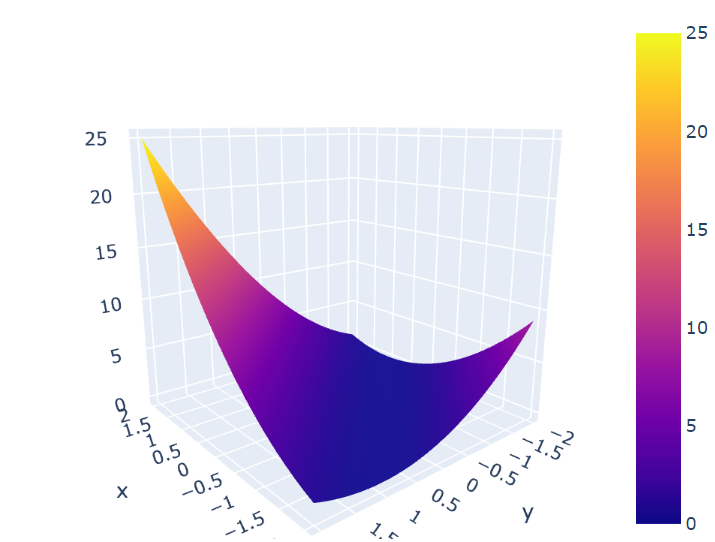
\includegraphics[width=12cm]{figures/SOFR/plot_G(x)_special_case.PNG}
    \caption{level Curve $G(\mathbf{x}_{t}) = k$, where all constants are set to one}
    \label{fig: plot_G(x)_SOFR_1M}
\end{figure}

\textbf{NB!} Figure \ref{fig: plot_G(x)_SOFR_1M}, is purely for illustration purposes, this will not be a realistic representation of $G(\mathbf{x}_{t})$. 
\\~\\
We will be interested in obtaining a minimum of $G(\mathbf{x}_{t})$, meaning that we will be interested in the following:  

\begin{align*}
\nabla G(\mathbf{x}_{t}) &= 
\left(
\partial_{x_{1}}G(\mathbf{x}_{t}), 
\partial_{x_{2}}G(\mathbf{x}_{t}), 
\partial_{x_{3}}G(\mathbf{x}_{t})
\right) 
\end{align*}

Where: 
\begin{align*}
\partial_{x_{1}}G(\mathbf{x}_{t}) &= 
-2q_{t}\alpha_{t} 
+ 2 \alpha_{t}^{2}x_{1}(t)  
+ 2\alpha_{t}\left[
\beta_{t} x_{2}(t)+ \gamma_{t} x_{3}(t)
\right] \\ 
\\
\partial_{x_{2}}G(\mathbf{x}_{t}) &=
-2q_{t}\beta_{t}
+ 2\beta_{t}^{2} x_{2}(t)
+ 2\beta_{t}\left[
\alpha_{t} x_{1}(t) + \gamma_{t} x_{3}(t)
\right] \\ 
\\ 
\partial_{x_{3}}G(\mathbf{x}_{t}) &=
-2q_{t}\gamma_{t}
+ 2\gamma_{t}^{2}x_{3}(t)
+ 2\gamma_{t}\left[
\alpha_{t} x_{1}(t) + \beta_{t} x_{2}(t)
\right]
\end{align*}

To verify that $G$ obtains a minimum we need the Hessian matrix $H(G)$ of $G$. This will be a $3\times 3$ matrix with entries:  

\begin{align*}
[H(G)]_{i,j} &= 
\frac{
\partial^{2}G
}{
\partial x_{i}\partial x_{j}
}, \; i=1,2,3,\;j=1,2,3
\end{align*}

Meaning that our Hessian matrix looks the following:
\begin{align*}
H(G) &= 
\begingroup
\renewcommand*{\arraystretch}{1.5}
\begin{bmatrix}
2\alpha_{t}^{2} & 
2\alpha_{t} \beta_{t} & 
2\alpha_{t} \gamma_{t} \\ 
2\alpha_{t} \beta_{t} &
2\beta_{t}^{2} &
2\beta_{t} \gamma_{t} \\
2\alpha_{t} \gamma_{t} &
2\beta_{t} \gamma_{t} & 
2\gamma_{t}^{2}
\end{bmatrix}
\endgroup
\end{align*}


Now as $\frac{\partial^{2}G(\mathbf{x}) }{\partial x_{i}^{2}} > 0$ for $i=1,2,3$ we know that the minimum should be obtained by setting $\partial_{x_{i}}G(\mathbf{x}) = 0$, i.e we must solve: 
\begin{align}
\label{eq: partial_derivative_equal_zero}
\nabla G(\mathbf{x}_{t}) = \mathbf{0}    
\end{align}

Now Equation \ref{eq: partial_derivative_equal_zero}, gives arise to the following matrix equation: 
\begin{align*}
\underbrace{
\begin{bmatrix}
\alpha_{t}^{2} & \alpha_{t}\beta_{t} & \alpha_{t}\gamma_{t} \\ 
\beta_{t}^{2} & \alpha_{t}\beta_{t} & \beta_{t}\gamma_{t} \\ 
\gamma_{t}^{2} & \alpha_{t}\gamma_{t} & \beta_{t}\gamma_{t}
\end{bmatrix}
}_{M}
\underbrace{
\begin{bmatrix}
x_{1}(t) \\ 
x_{2}(t) \\ 
x_{3}(t)
\end{bmatrix}
}_{\mathbf{x}_{t}}
&= 
\underbrace{
q 
\begin{bmatrix}
\alpha_{t} \\ 
\beta_{t} \\ 
\gamma_{t} 
\end{bmatrix}
}_{\mathbf{b}}
\iff  
M\mathbf{x}_{t} = \mathbf{b}
\end{align*}

Now: 
\begin{align*}
\det(M) &= 
\alpha_{t}^{2}\left[
\alpha_{t}\beta_{t}^{2}\gamma_{t} - \alpha_{t}\beta_{t}\gamma_{t}^{2}
\right]
- \alpha_{t}\beta_{t}\left[
\beta_{t}^{3}\gamma_{t} - \beta_{t}\gamma_{t}^{3}
\right]
+ \alpha_{t}\gamma_{t}\left[
\beta_{t}^{2}\alpha_{t}\gamma_{t} -\alpha_{t}\beta_{t}\gamma_{t}^{2}
\right] \\ 
&= 
\alpha_{t}\beta_{t}\gamma_{t}(\beta_{t}-\gamma_{t})\left[
\alpha_{t}(\alpha_{t}+\gamma_{t}) -\beta_{t}(\beta_{t} + \gamma_{t})
\right]
\end{align*}

In order for $\det(M) \neq 0$, we must have:
\begin{empheq}[box=\fbox]{align}
\alpha_{t} &\neq 0, \; \beta_{t} \neq 0, \; \gamma_{t} \neq 0  \nonumber
\\
\beta_{t} &\neq \gamma_{t}, \; \gamma_{t} \neq -(\alpha_{t} + \beta_{t}) \label{eq: condition_det(M)_not_zero}
\end{empheq}

%Assume that the necessary conditions in \ref{eq: condition_det(A)_not_zero} holds, we then get, that the inverse is %given by: 


Thus the optimal weight $\hat{\mathbf{x}}_{t}$ will then be:   
\begin{align*}
\hat{\mathbf{x}}_{t} &= 
M^{-1}\mathbf{b}
\end{align*}


Now if the Condition \ref{eq: condition_det(M)_not_zero} does not hold, one approach could be:

\begin{align}
\label{eq: Basis_Pursuit_lp}
\begin{array}{ll@{}ll}
\text{minimize}  & \displaystyle\sum\limits_{i=1}^{3}x_{i}(t)&  &\\
\text{subject to}& \displaystyle   M\mathbf{x}_{t} = & \mathbf{b}
\end{array}    
\end{align}

Assume that $\Tilde{\mathbf{x}}_{t}$ is the optimal solution to \ref{eq: Basis_Pursuit_lp}, this method is
very much related to Basis Pursuit \cite{chen1998atomic}.



\newpage 

\subsection{Simulation of Error distribution}

To say something about how good the hedge in Proposition \ref{prop: optimal_hedge_arithmetic_3M_geometric}, we study: 
\begin{align*}
ER_{1}(t) :&= X^{3M_{A}}(S,T) - \hat{a}_{t}^{3M}f^{3M}(t,S,T) \\ 
&= \frac{1}{T-S}\int_{S}^{T}r(u)du - \frac{1}{T-S}\int_{S}^{T}\E_{Q}[r(u)|\F_{t}]du \\ 
&= 
\frac{1}{T-S}\left(
\int_{S}^{T}r(u)du - \int_{S}^{T}\E_{Q}[r(u)|\F_{t}]du
\right)
\end{align*}

We will also study the Error distribution from Section \ref{sec: 3M_A_vs_(a,b,c)_1M_SOFR}, now this will correspond to: 
\begin{align*}
ER_{2}(t) &= 
X^{3M_{A}}(S,T) - \left(
\hat{a}_{t}f^{1M}(t,S,T_{1M}) + 
\hat{b}_{t}f^{1M}(t,T_{1M}, T_{2M}) + 
\hat{c}_{t}f^{1M}(t,T_{2M}, T)
\right)
\end{align*}


We choose the Vasicek model for simulation:
\begin{align*}
dr(t) &= \alpha[m-r(t)]dt + \sigma dW^{Q}(t)    
\end{align*}

For calculating $X^{3M_{A}}(S,T)$, we use the closed expression for $\int_{S}^{T}r(u)du$  as described in Equation \ref{eq: Vasicek_closed_expr_3M_SOFR} p.\pageref{eq: Vasicek_closed_expr_3M_SOFR}:

\begin{align*}
\int_{S}^{T}r(u)du 
&= 
\left(
\frac{r(t)-m}{\alpha}
\right)
\left[
e^{-\alpha(S-t)} - e^{-\alpha(T-t)}
\right]
+ m(T-S) 
+ 
\frac{\sigma}{\alpha}\int_{t}^{T}\Sigma(u,t,S,T)dW^{Q}(u)
\end{align*}

Where: 
\begin{align*}
\Sigma(u,t,S,T) &= 
\left[
e^{-\alpha(S-u)}-e^{-\alpha(T-u)}
\right]\mathbbm{1}_{[t,S)}(u) 
+ 
\left[
1-e^{-\alpha(T-u)}
\right]\mathbbm{1}_{[S,T]}(u)
\end{align*}


For simplicity we fix $t=0$, meaning that we will study: 
$ER_{1}(0)$ and $ER_{2}(0)$, using the Vasicek model, where the parameters are as shown below:

\begin{figure}[htp]
    \centering
    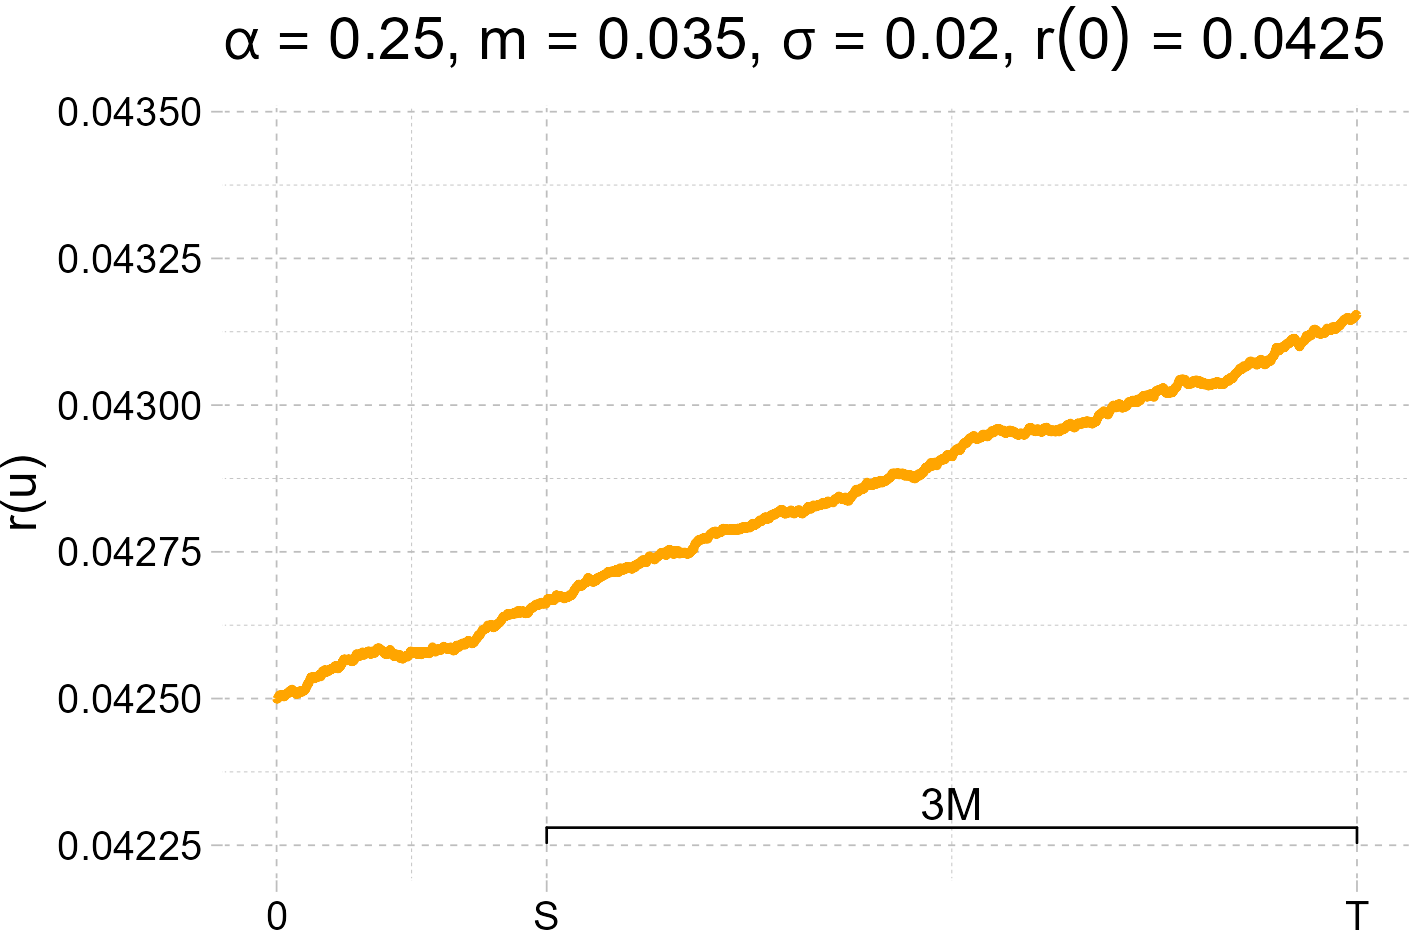
\includegraphics[width=12cm]{figures/SOFR/Vasicek_path.png}
    \caption{Path of Vasicek model for $u\in [0,T]$}
    \label{fig: Vasicek_path}
\end{figure}

\newpage 
\textbf{3M-arithmetic vs $\hat{a}_{0}^{3M}$ 3M-SOFR futures calculations:}
\\~\\
We have that: 
\begin{align*}
\hat{a}_{t}^{3M} = \frac{
\int_{S}^{T}\E_{Q}[r(u)|\F_{t}]du
}{
(T-S)f^{3M}(t,S,T)
}    
\end{align*}

For calculating $f^{3M}(t,S,T)$ we have from 
Equation \ref{eq: Vasicek_3M_SOFR_closed_formula} p.\pageref{eq: Vasicek_3M_SOFR_closed_formula}, that:  
\begin{align*}
f^{3M}(t,S,T) &= 
\frac{1}{T-S}\left[
\exp\left(
A(t,S,T) + B(t,S,T)r(t)
\right)
-1
\right]
\end{align*}

Where: 
\begin{align*}
A(t,S,T) &= m(T-S) - \frac{m}{\alpha}\left[
e^{-\alpha(S-t)} - e^{-\alpha(T-t)}
\right] + \frac{1}{2}\frac{\sigma^{2}}{\alpha^{2}}\int_{t}^{T}\Sigma^{2}(u,t,S,T)du \\
B(t,S,T) &= \frac{1}{\alpha}\left[
e^{-\alpha(S-t)} - e^{-\alpha(T-t)}
\right]
\end{align*}

We are interested in the case where $t=0$, giving us:
\begin{align*}
\hat{a}_{0}^{3M} = \frac{
\int_{S}^{T}\E_{Q}[r(u)]du
}{
(T-S)f^{3M}(0,S,T)
}
= 0.995
\end{align*}

\textbf{3M-arithmetic vs $(\hat{a}_{0}, \hat{b}_{0}, \hat{c}_{0})$ 1M-SOFR futures calculations}
\\~\\
In this simulation we had that Condition \ref{eq: condition_det(M)_not_zero} were met, as we got:
\begin{align*}
\alpha_{0} &= 0.0423 \\ 
\beta_{0} &= 0.0421 \\ 
\gamma_{0} &= 0.0420
\end{align*}

Furthermore, the optimal weight $\hat{\mathbf{x}}_{0}$ turned out to be:
\begin{align*}
\hat{\mathbf{x}}_{0} &= 
\begin{bmatrix}
\alpha_{0}^{2} & \alpha_{0}\beta_{0} & \alpha_{0}\gamma_{0} \\ 
\beta_{0}^{2} & \alpha_{0}\beta_{0} & \beta_{0}\gamma_{0} \\ 
\gamma_{0}^{2} & \alpha_{0}\gamma_{0} & \beta_{0}\gamma_{0}
\end{bmatrix}^{-1}
\begin{bmatrix}
q_{0}\alpha_{0} \\ 
q_{0}\beta_{0} \\ 
q_{0}\gamma_{0}
\end{bmatrix}
=
\begin{bmatrix}
0.501 \\
0.501 \\
-0.004
\end{bmatrix} 
\end{align*}

Here:
\[
q_{0} = \E_{Q}[X^{3M_{A}}(S,T)] = 0.0421
\]


\newpage


\textbf{3M-arithmetic vs 3M-geometric SOFR futures:}

\begin{figure}[htp]
    \centering
    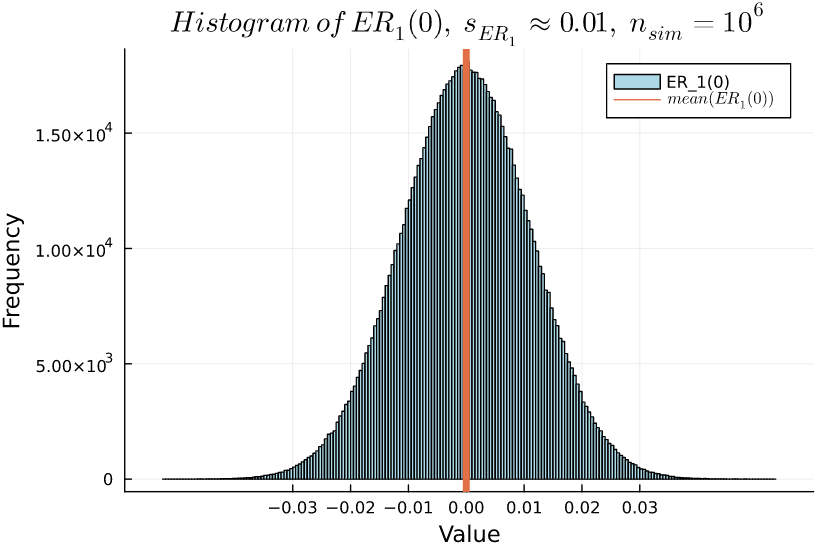
\includegraphics[width=12cm]{figures/SOFR/ER_1(0).PNG}
    \caption{Simulation of $ER_{1}(0)$}
    \label{fig: ER_1_(0)}
\end{figure}

Here we see the distribution $ER_{1}(0)$, we see that the mean of $ER_{1}(0)$, $\overline{ER_{1}(0)} = 0$, this indicates that one average hedging $X^{3M_{A}}(S,T)$ where one takes $\hat{a}_{0} = 0.995$-positions in $3M$-SOFR futures would be a good hedge. We also have that $\E_{Q}[ER_{1}(0)] = 0$.  
\\~\\
\textbf{3M-arithmetic vs $(\hat{a}_{0}, \hat{b}_{0}, \hat{c}_{0})$ 1M-SOFR futures}

\begin{figure}[htp]
    \centering
    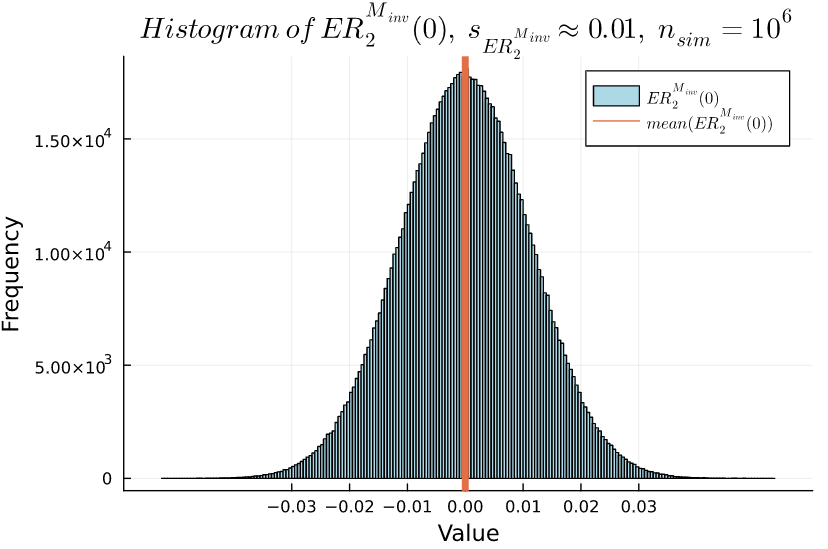
\includegraphics[width=12cm]{figures/SOFR/ER_2(0)_M_inv.PNG}
    \caption{Simulation of $ER_{2}^{inv}(0)$}
    \label{fig: ER_2_(0)_M_inv}
\end{figure}

Here we see the $ER_{2}(0)$ distribution under the assumption that $M$ is invertible. Here we have taken the following position in $1M$-SOFR futures: 
\[
(\hat{a}_{0}, \hat{b}_{0}, \hat{c}_{0})
= 
(0.501, 0.501, -0.004)
\]
We see that the mean of $ER_{2}^{M_{inv}}(0)$, $\overline{ER_{2}^{M_{inv}}(0)} = 0$, which then again indicated that on average taking the above position at time $t=0$ would be a good hedge. 
\\~\\
\begin{comment}
To illustrate the need for an optimal position, let us naively choose a strategy. We deal with futures rates to ease the intuition think of cash settlements. Consider the case when you have a 30 Million dollar loan in which one pays a floating 3M arithmetic average. 
\end{comment}
To illustrate this a bit further, we can take a look at the error distribution where one naively chooses a strategy in 1M-SOFR futures, for instance, the following weighting: 
\[
(\hat{a}_{0}, \hat{b}_{0}, \hat{c}_{0})
= 
(0.33, -0.33, 0.33)
\]

\begin{figure}[htp]
    \centering
    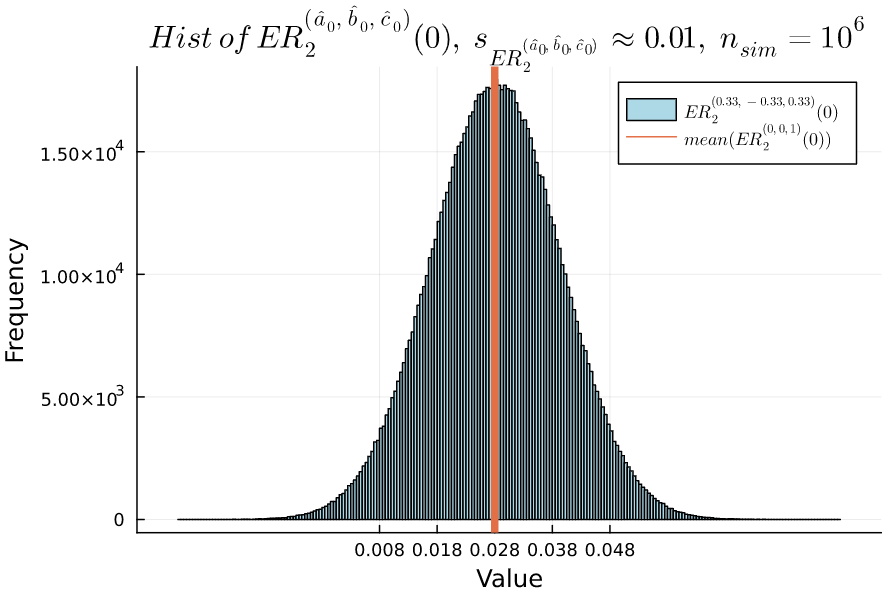
\includegraphics[width=12cm]{figures/SOFR/ER_2(0)_random.PNG}
    \caption{Simulation of $ER_{2}^{(\hat{a}_{0}, \hat{b}_{0}, \hat{c}_{0})}(0)$}
    \label{fig: ER_2_(0)_random}
\end{figure}

Now, the weights that we have calculated are weighing in SOFR futures rates, not the actual position one would take at CME, from earlier we remember that SOFR futures at CME are quoted the following way (modified to our example with decimals): 
\begin{align*}
Q^{\ell M}(t,S,T) &= 1- f^{\ell M}(t,S,T),\; \ell = 1, 3 
\end{align*}

To get more intuition about the weighing in SOFR futures, we construct an example:

\begin{example}
Assume that we have a loan of 30 million over a 3M period. From the contract, it is agreed upon that the rate we will pay is the floating 3M-arithmetic rate $X^{3M_{A}}(S,T)$ plus an additional risk-premium of $200$ bp (basis points). 
\\~\\
We want to hedge against rising interest rates, so if $f^{\ell M}$ increases, then $Q^{\ell M}$ decreases. 
\\~\\
\textbf{Case 1:} Hedge by taking position in 3M-SOFR futures. From previous calculations, we got $\hat{a}_{0}^{3M} = 0.995$. This will correspond to the position in the 3M SOFR futures rate. Now a 3M SOFR futures are based upon a notional of 1 million dollars. Meaning that we would need 30 contracts to cover our loan amount. We can not take a fractional position, meaning that we, in this case, would take one position in the futures rate. Since we want to hedge against rising interest rates, we would take 30 short positions here. 

\newpage
\textbf{Case 2:} Hedge by taking position in 1M-SOFR futures. From our simulation we got $(\hat{a}_{0}, \hat{b}_{0}, \hat{c}_{0})
= 
(0.501, 0.501, -0.004) \approx (0.5, 0.5, 0.0)
$. Now 1M-SOFR futures has a notional of 5 million dollars. So to cover our loan, we would need six contracts. These would be covered by taking three positions in the first futures contract, three in the middle futures contract, and zero in the last. The type of position would be a short position. 
\end{example}


We see that for all our simulations, the error distributions seem to be normally distributed. This is not surprising as in each simulation, and we take a normal random variable: $\int_{S}^{T}r(u)du$ as described in  Equation \ref{eq: Vasicek_closed_expr_3M_SOFR} p.\pageref{eq: Vasicek_closed_expr_3M_SOFR}, and subtract a constant/linear combination of constants. This is a new, normally distributed random variable with an altered mean. 
We can also address the normality via a QQplot:


\begin{figure}[htp]
    \centering
    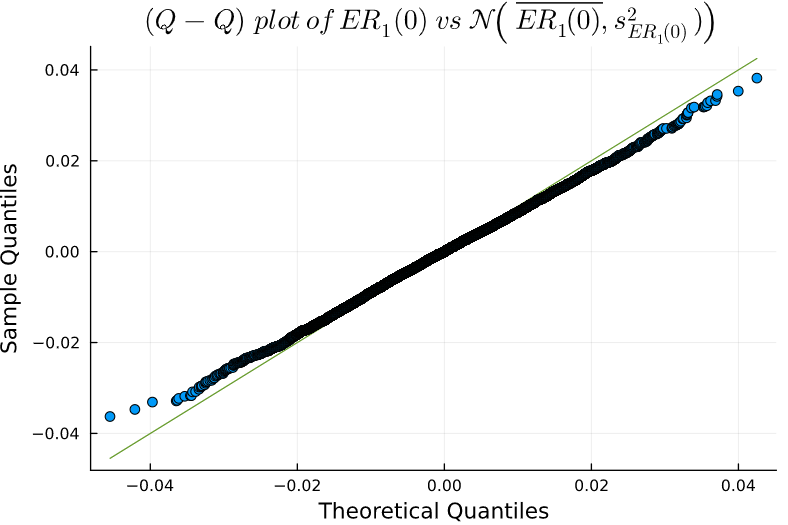
\includegraphics[width=10cm]{figures/SOFR/QQ_plot_ER_1(0).PNG}
    \caption{(Q-Q) plot of $ER_{1}(0)$}
    \label{fig: ER_1(0)_QQ_plt}
\end{figure}
